\documentclass[a4paper,12pt]{article}
\usepackage[margin=.9in]{geometry}
\usepackage{graphicx}
\usepackage{parskip}
%\usepackage{titling}
\usepackage[utf8]{inputenc}
\usepackage{tikz}
\usetikzlibrary{shapes.geometric, arrows}
\graphicspath{ {images/} }

\tikzstyle{module} = [rectangle, rounded corners, minimum width=2cm, minimum height=1.2cm,text centered, draw=black, fill=red!30, text width=3.5cm]

\tikzstyle{startstop} = [rectangle, rounded corners, minimum width=1.5cm, minimum height=.8cm,text centered, draw=black, fill=red!30]
\tikzstyle{io} = [trapezium, trapezium left angle=70, trapezium right angle=110, minimum width=1cm, minimum height=.8cm, text centered, draw=black, fill=blue!30, inner sep=.2cm]
\tikzstyle{process} = [rectangle, minimum width=3cm, minimum height=.8cm, text centered, draw=black, fill=orange!30, text width=3.5cm]
\tikzstyle{decision} = [diamond, minimum width=3cm, minimum height=.8cm, text centered, draw=black, fill=green!30, text width=1.8cm, aspect=1.8, inner sep=0]
\tikzstyle{arrow} = [thick,->,>=stealth]

\begin{document}
\begin{titlepage}
    \begin{center}
        \vspace*{1cm}
        
        \Huge
        \textbf{Technical Specification}
        
        \vspace{0.5cm}
        \LARGE
        SDP Group 15-H
        
        \vspace{1.5cm}
        \normalsize
        Julijonas Kikutis\\ 
		Patrick Green\\
		Aseem Narang\\
		Ankit Sonkar\\
		David McArthur\\
		Emilia Bogdanova
        
        \vfill
        
        
        \vspace{0.8cm}
        
        \begin{figure}
    	\vspace*{-3em}
    	\centering
    	
\includegraphics[scale=.30]{logo.png}
		\end{figure}
        
        \Large
        University of Edinburgh\\
        
    \end{center}
\end{titlepage}

\tableofcontents

\newpage

\section{System architecture}

Venus has gone through several stages of changes. The earliest prototype had four regular wheels as seen in Figure \ref{fig:robot0}. This made us realise that we have to keep in mind the space
constraints when building the base as we need to accommodate not only the motors
for the wheels but also the kicking and grabbing mechanism. 
\\The next, more sophisticated design, was a robot with four powerful kickers that used elastics as seen in Figure \ref{fig:robot3}. The idea was to stretch elastics for all four kickers using the star shape element on top of the robot as seen in the picture and then release. This gave a lot of energy to the ball. However, this design had a disadvantage because the robot was not able to kick the ball for varying distances, which was an essential requirement for the first milestone. Moreover, the dimensions of the robot were exceeding the maximum size limits and the speed of the ball was exceeding the one allowed in the game rules. 

\begin{figure}[h]
	\centering
	\begin{minipage}[b]{.48\textwidth}
        \centering
		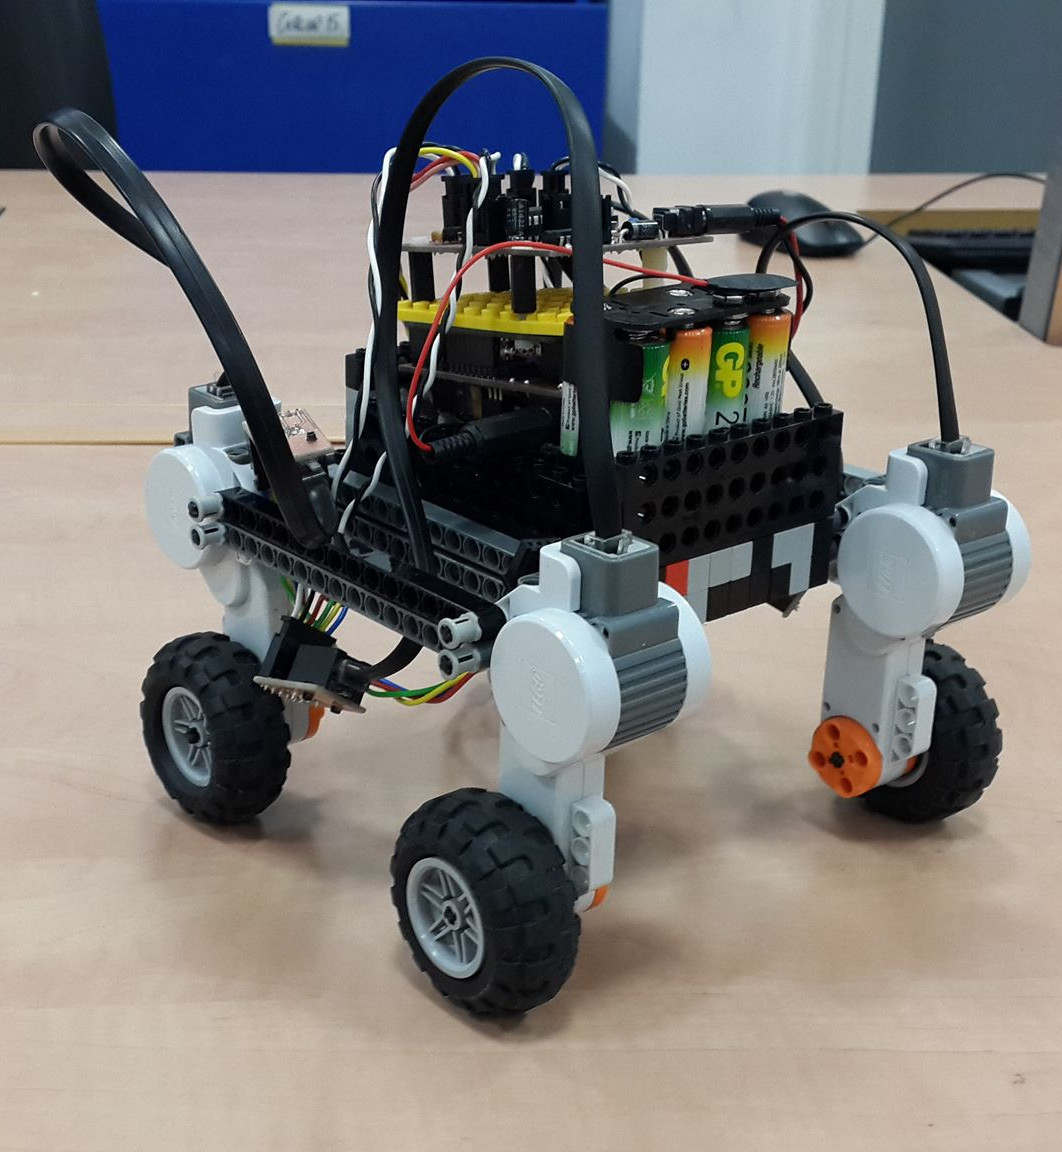
\includegraphics[scale=.18]{robot0.jpg}
		\caption{The first prototype}
		\label{fig:robot0}
	\end{minipage}
	~
	\begin{minipage}[b]{.48\textwidth}
        \centering
		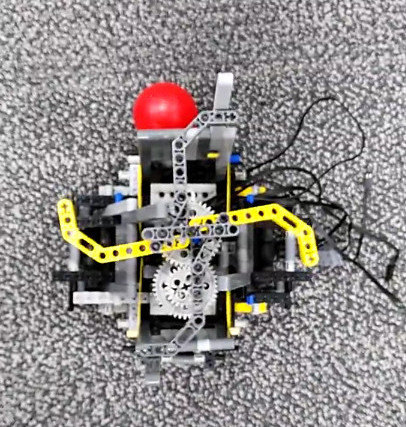
\includegraphics[scale=.65]{robot3.jpg}
		\caption{The robot with four kickers}
		\label{fig:robot3}
	\end{minipage}
\end{figure}

Taking all the disadvantages of previous designs into account we came up with a new design as seen in Figures \ref{fig:open} and \ref{fig:closed}. Advantage of this design is that it is simple and at the same time the robot can still move fast enough to play football and the power of the kicks can be precisely controlled. 

The grabbing mechanism for this design went through two iterations of development.
The first grabber we developed was falling down on the ball in order to catch it, thus was deemed not suitable because it obstructed the ball more than it was allowed by the football game rules. Venus also had difficulties at placing the ball in front of the kicker at initial kicking position, because the grabber pushed it
too far inside the kicker. Thus, the grabber was replaced by the newer design depicted in Figure \ref{fig:open} which has two symmetrical grabbers that interlock when the robot is moving to conserve space and are able to reach a more distant ball.

\begin{figure}[ht]
	\centering
	\begin{minipage}[b]{.48\textwidth}
        \centering
		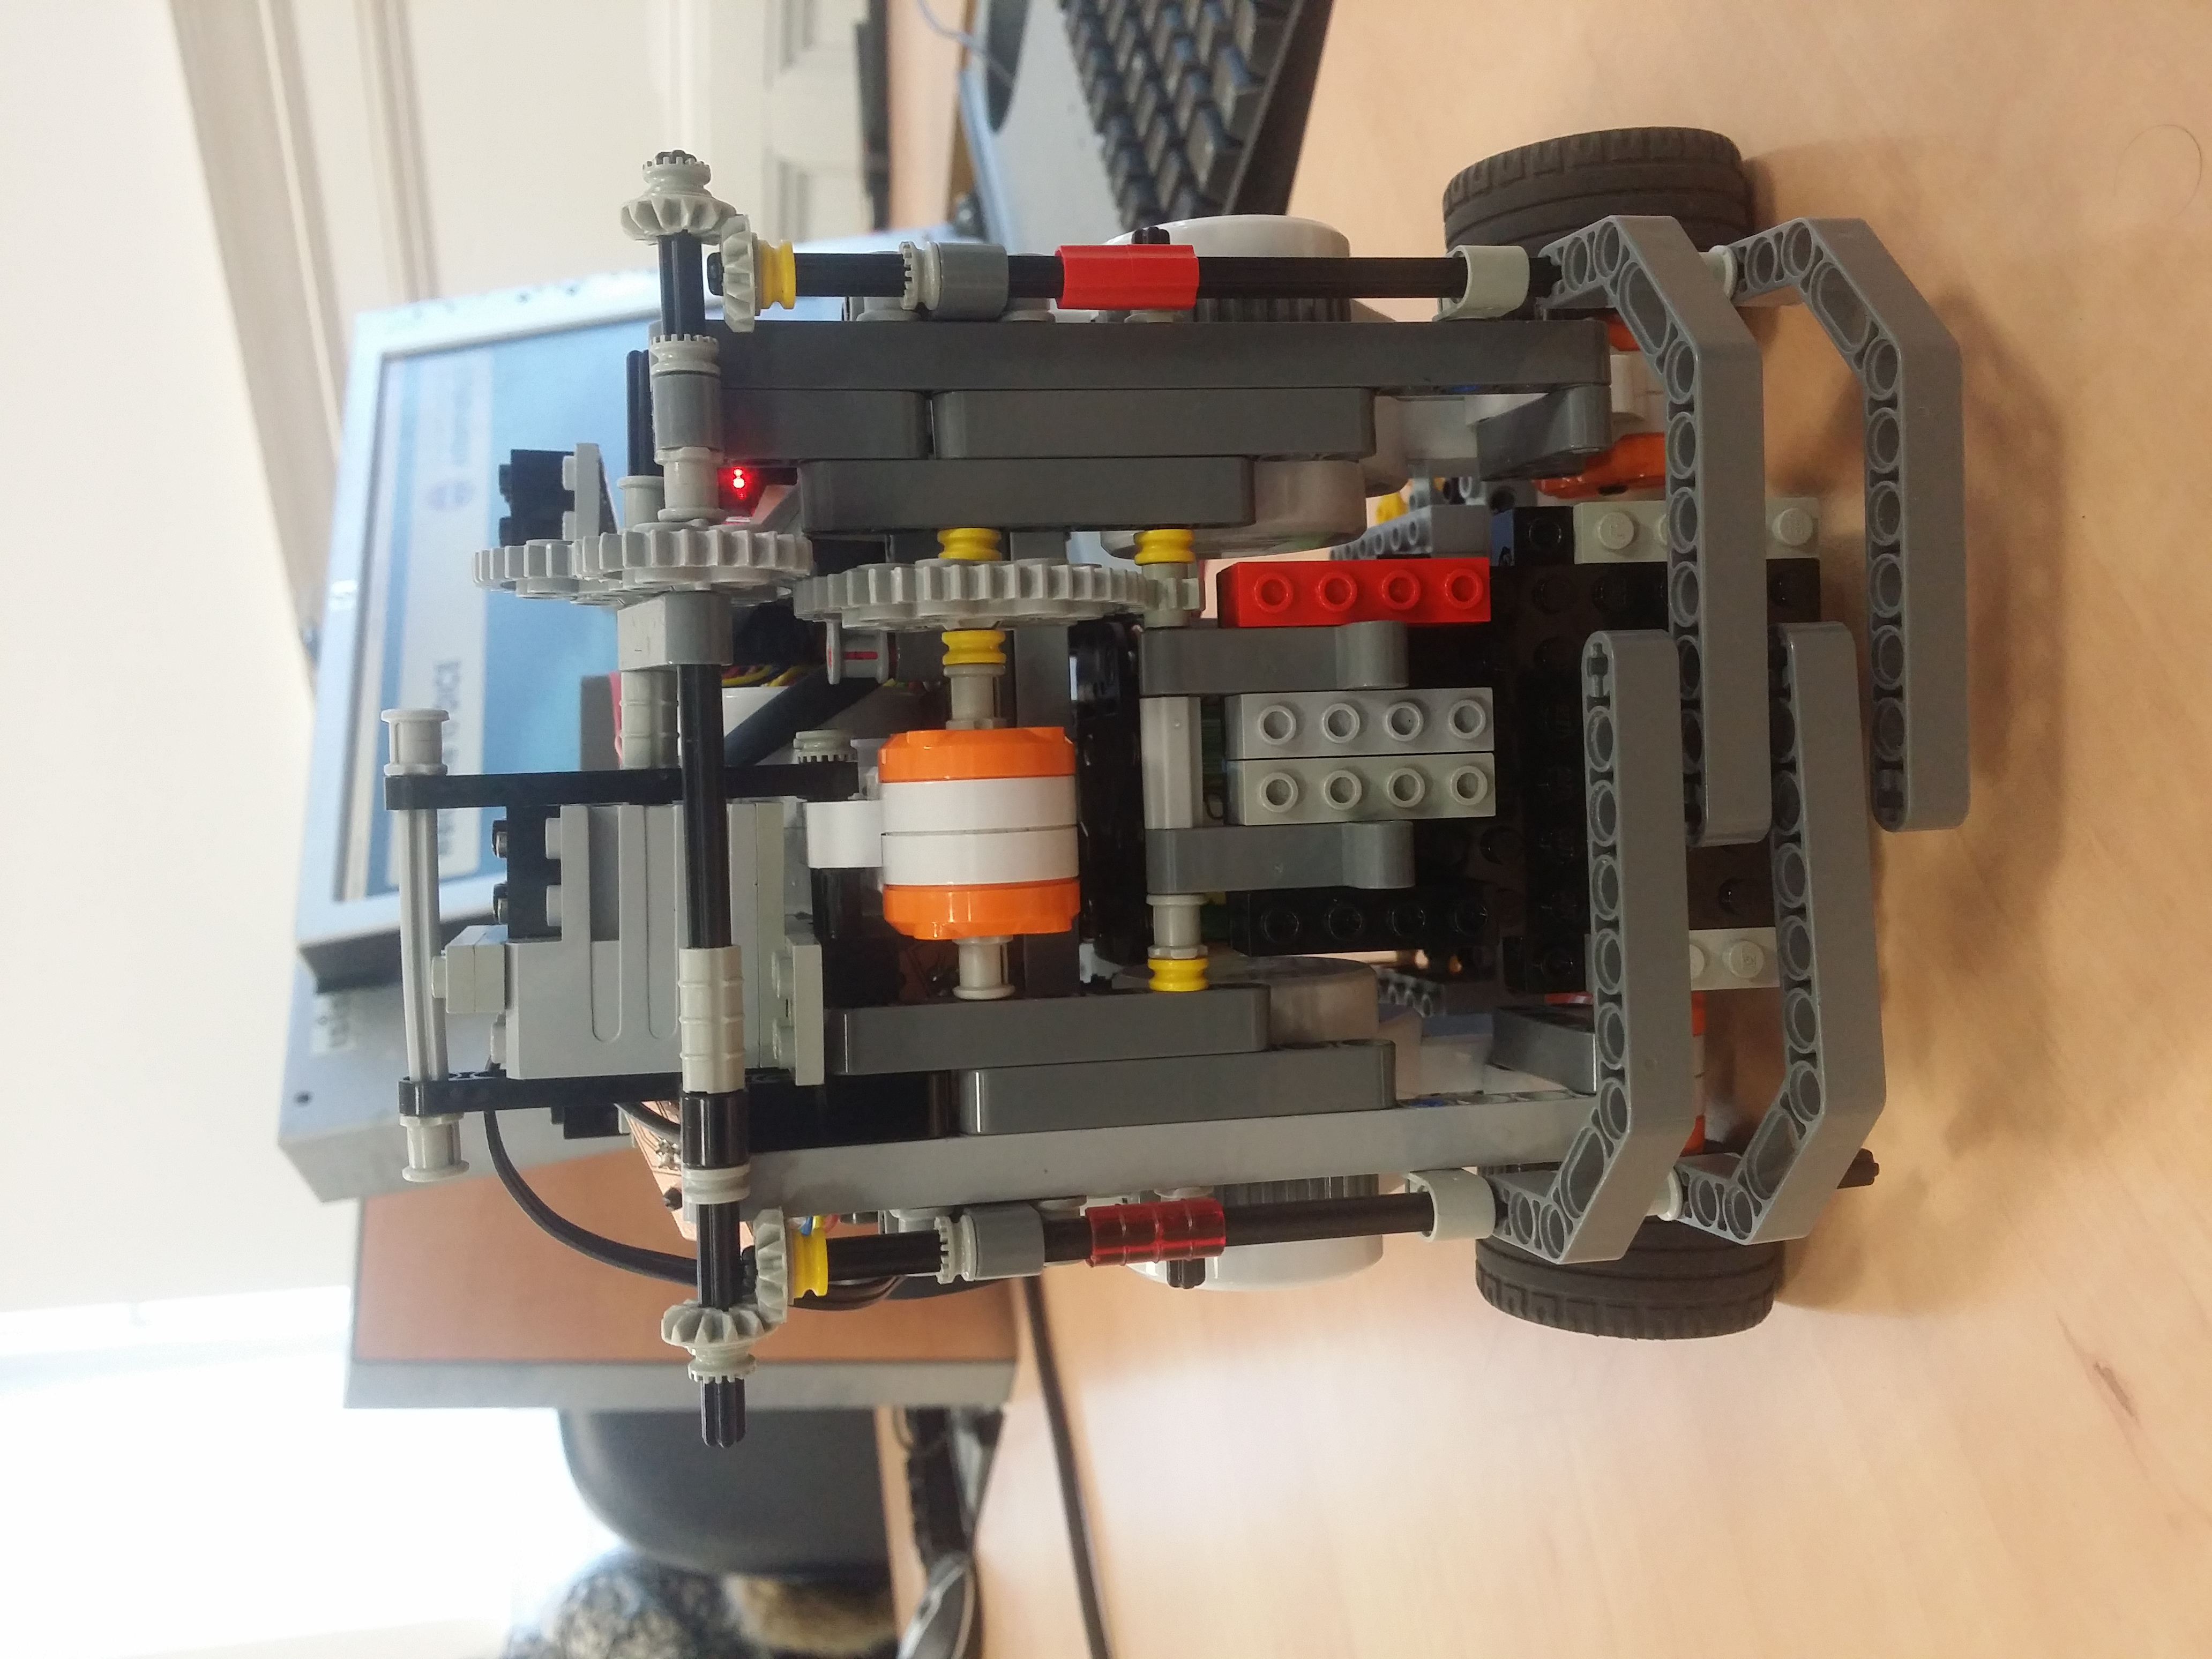
\includegraphics[scale=0.065, angle=-90]{closed_front.jpg}
		\caption{With grabber in closed position}
		\label{fig:closed}
	\end{minipage}
	~
	\begin{minipage}[b]{.48\textwidth}
        \centering
		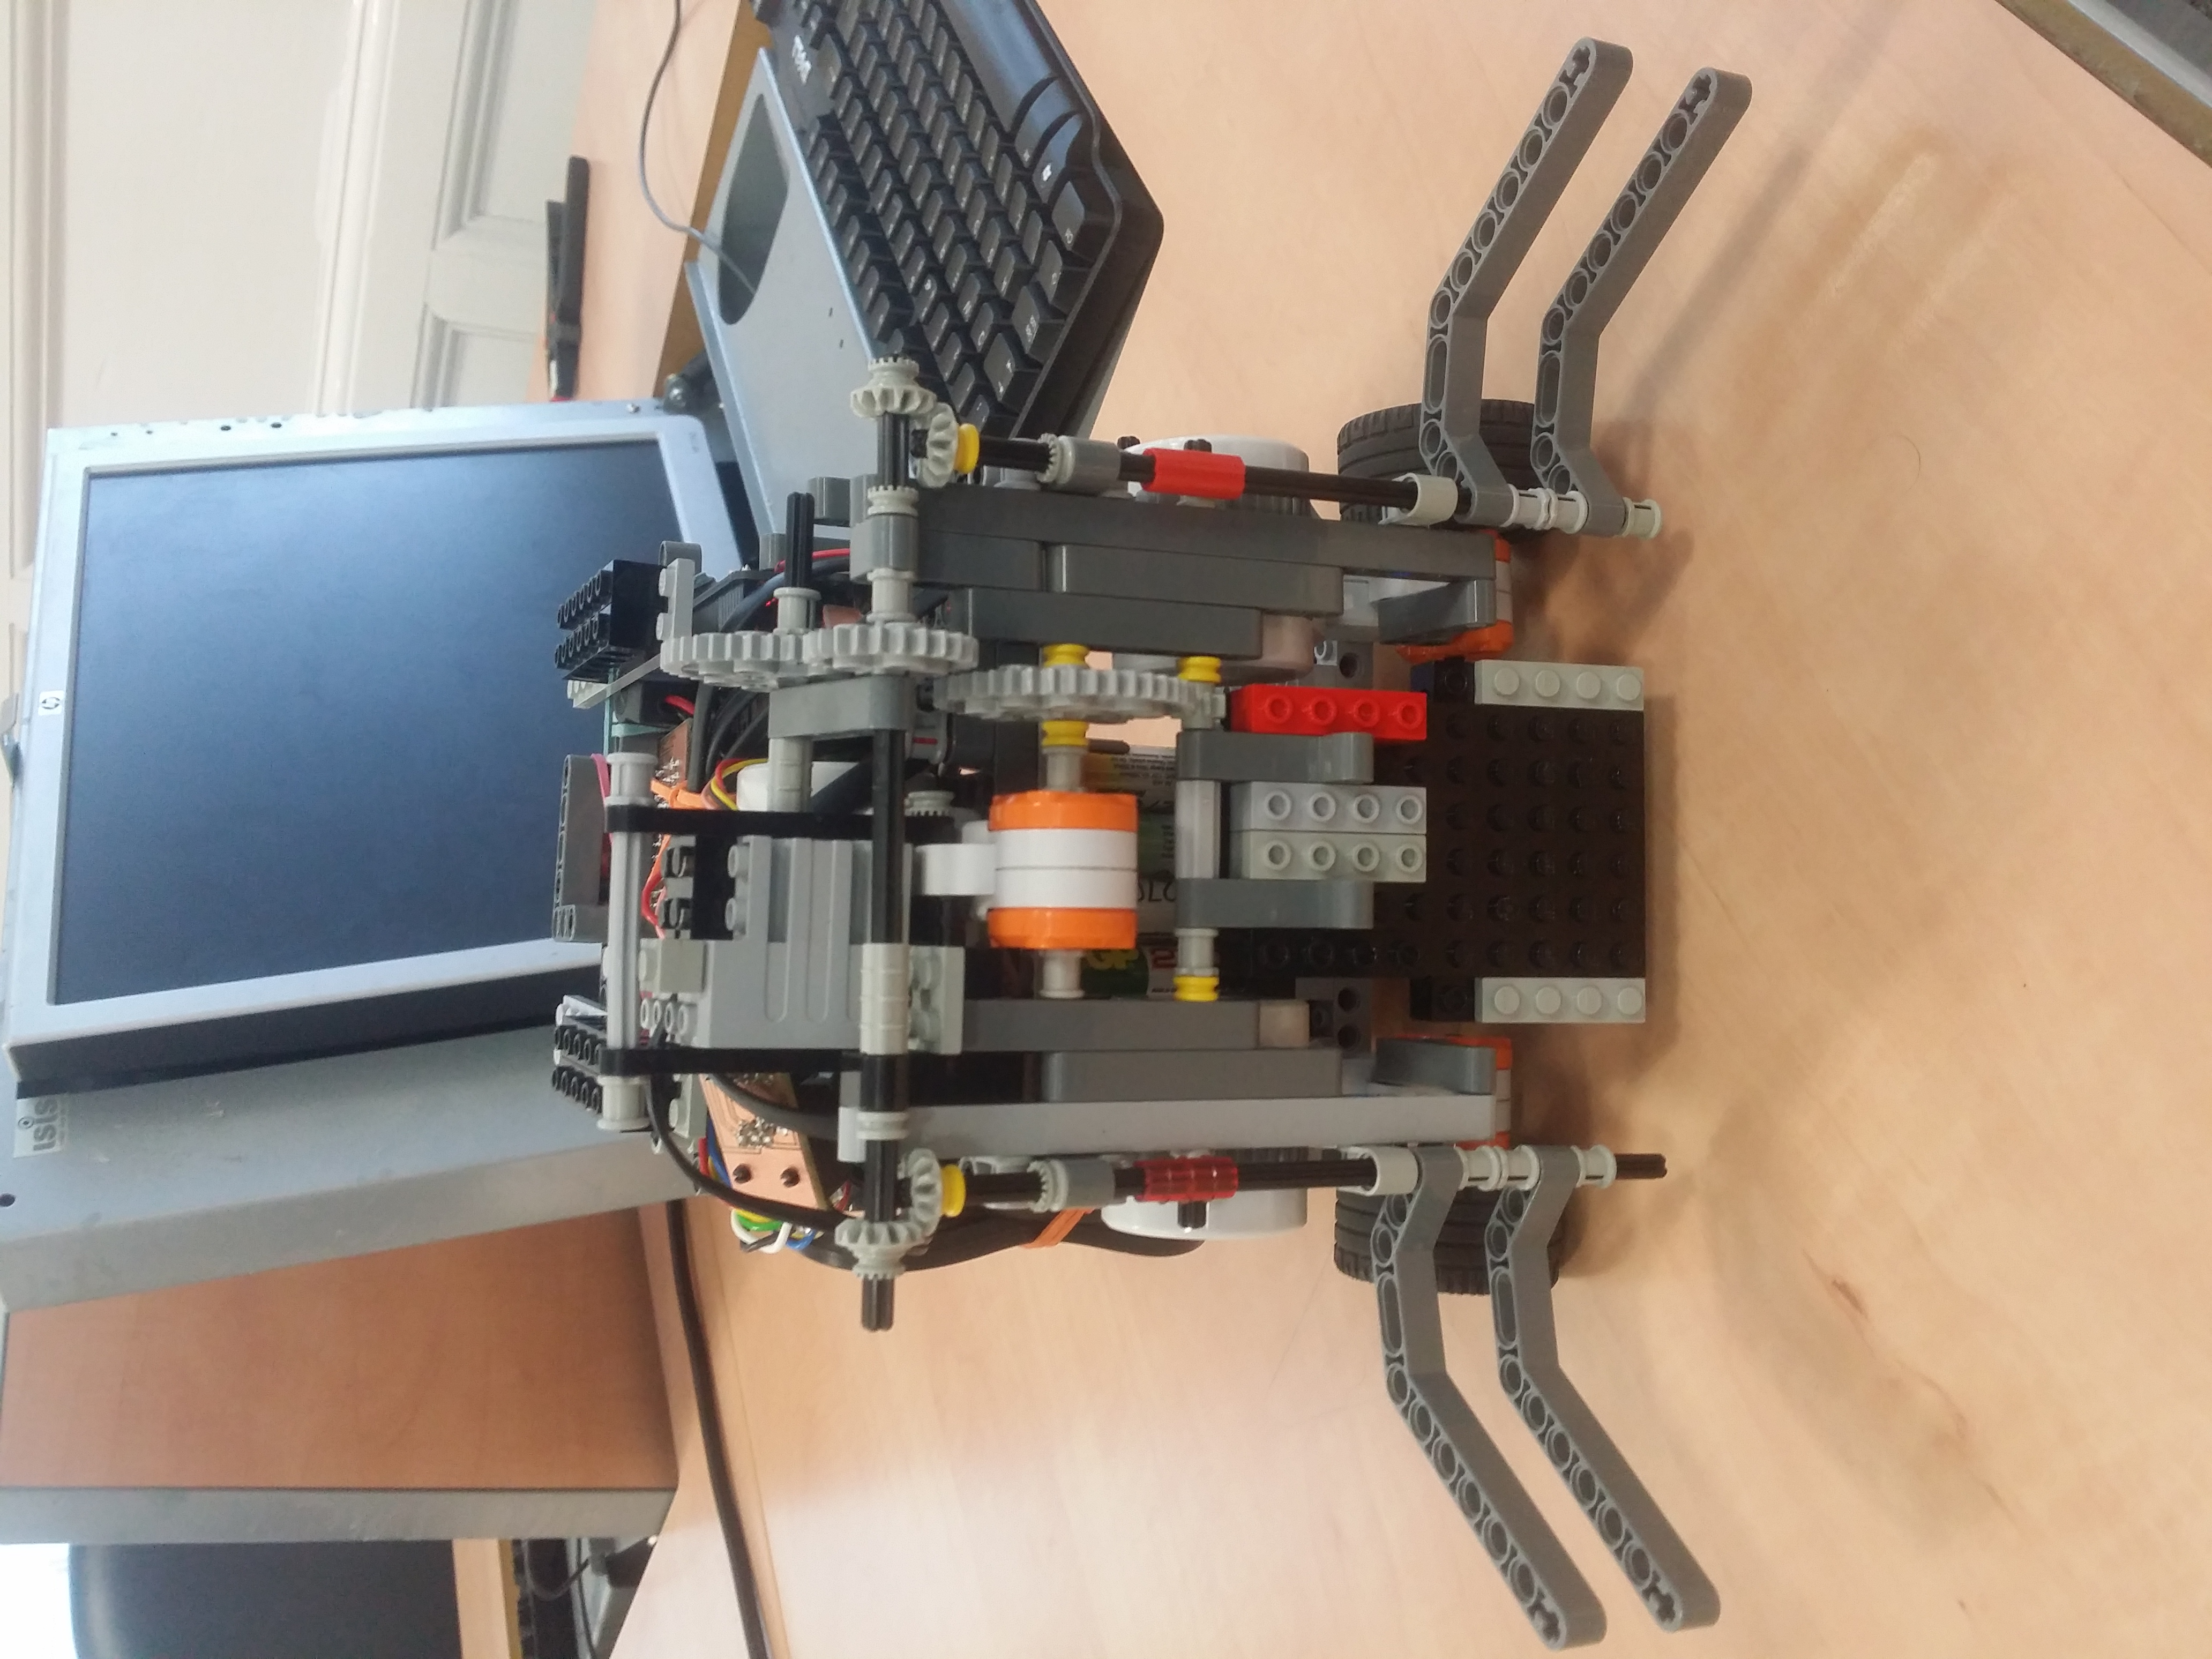
\includegraphics[scale=0.065, angle=-90]{grab_open.jpg}
		\caption{With grabber in open position}
		\label{fig:open}
	\end{minipage}
\end{figure}

After playing the first friendly, we have realized that Venus isn't fast enough comparing to other robots. We decided to start the design from scratch again. Our latest design has four holonomic wheels, which allow Venus to move fast and also in different directions (Figure FIGURE). We had also refused of using any kickers, because none of the kickers we thought of, could fit with four NXT motors. Venus kicks using its grabber and spinning action. The design of the grabber hasn't changed much from the previous time. 

When we were satisfied with the look of Venus, we also made all cables look neat using elastics. We also ensured that we can still access the battery pack and Arduino board if needed as seen in Figure \ref{fig:battery}.

\begin{figure}
	\centering
	\begin{minipage}[b]{.48\textwidth}
        \centering
		\includegraphics[scale=.065]{battery1.jpg}
		\caption{Battery pack easily accessible}
		\label{fig:battery}
	\end{minipage}
	~
	\begin{minipage}[b]{.48\textwidth}
        \centering
		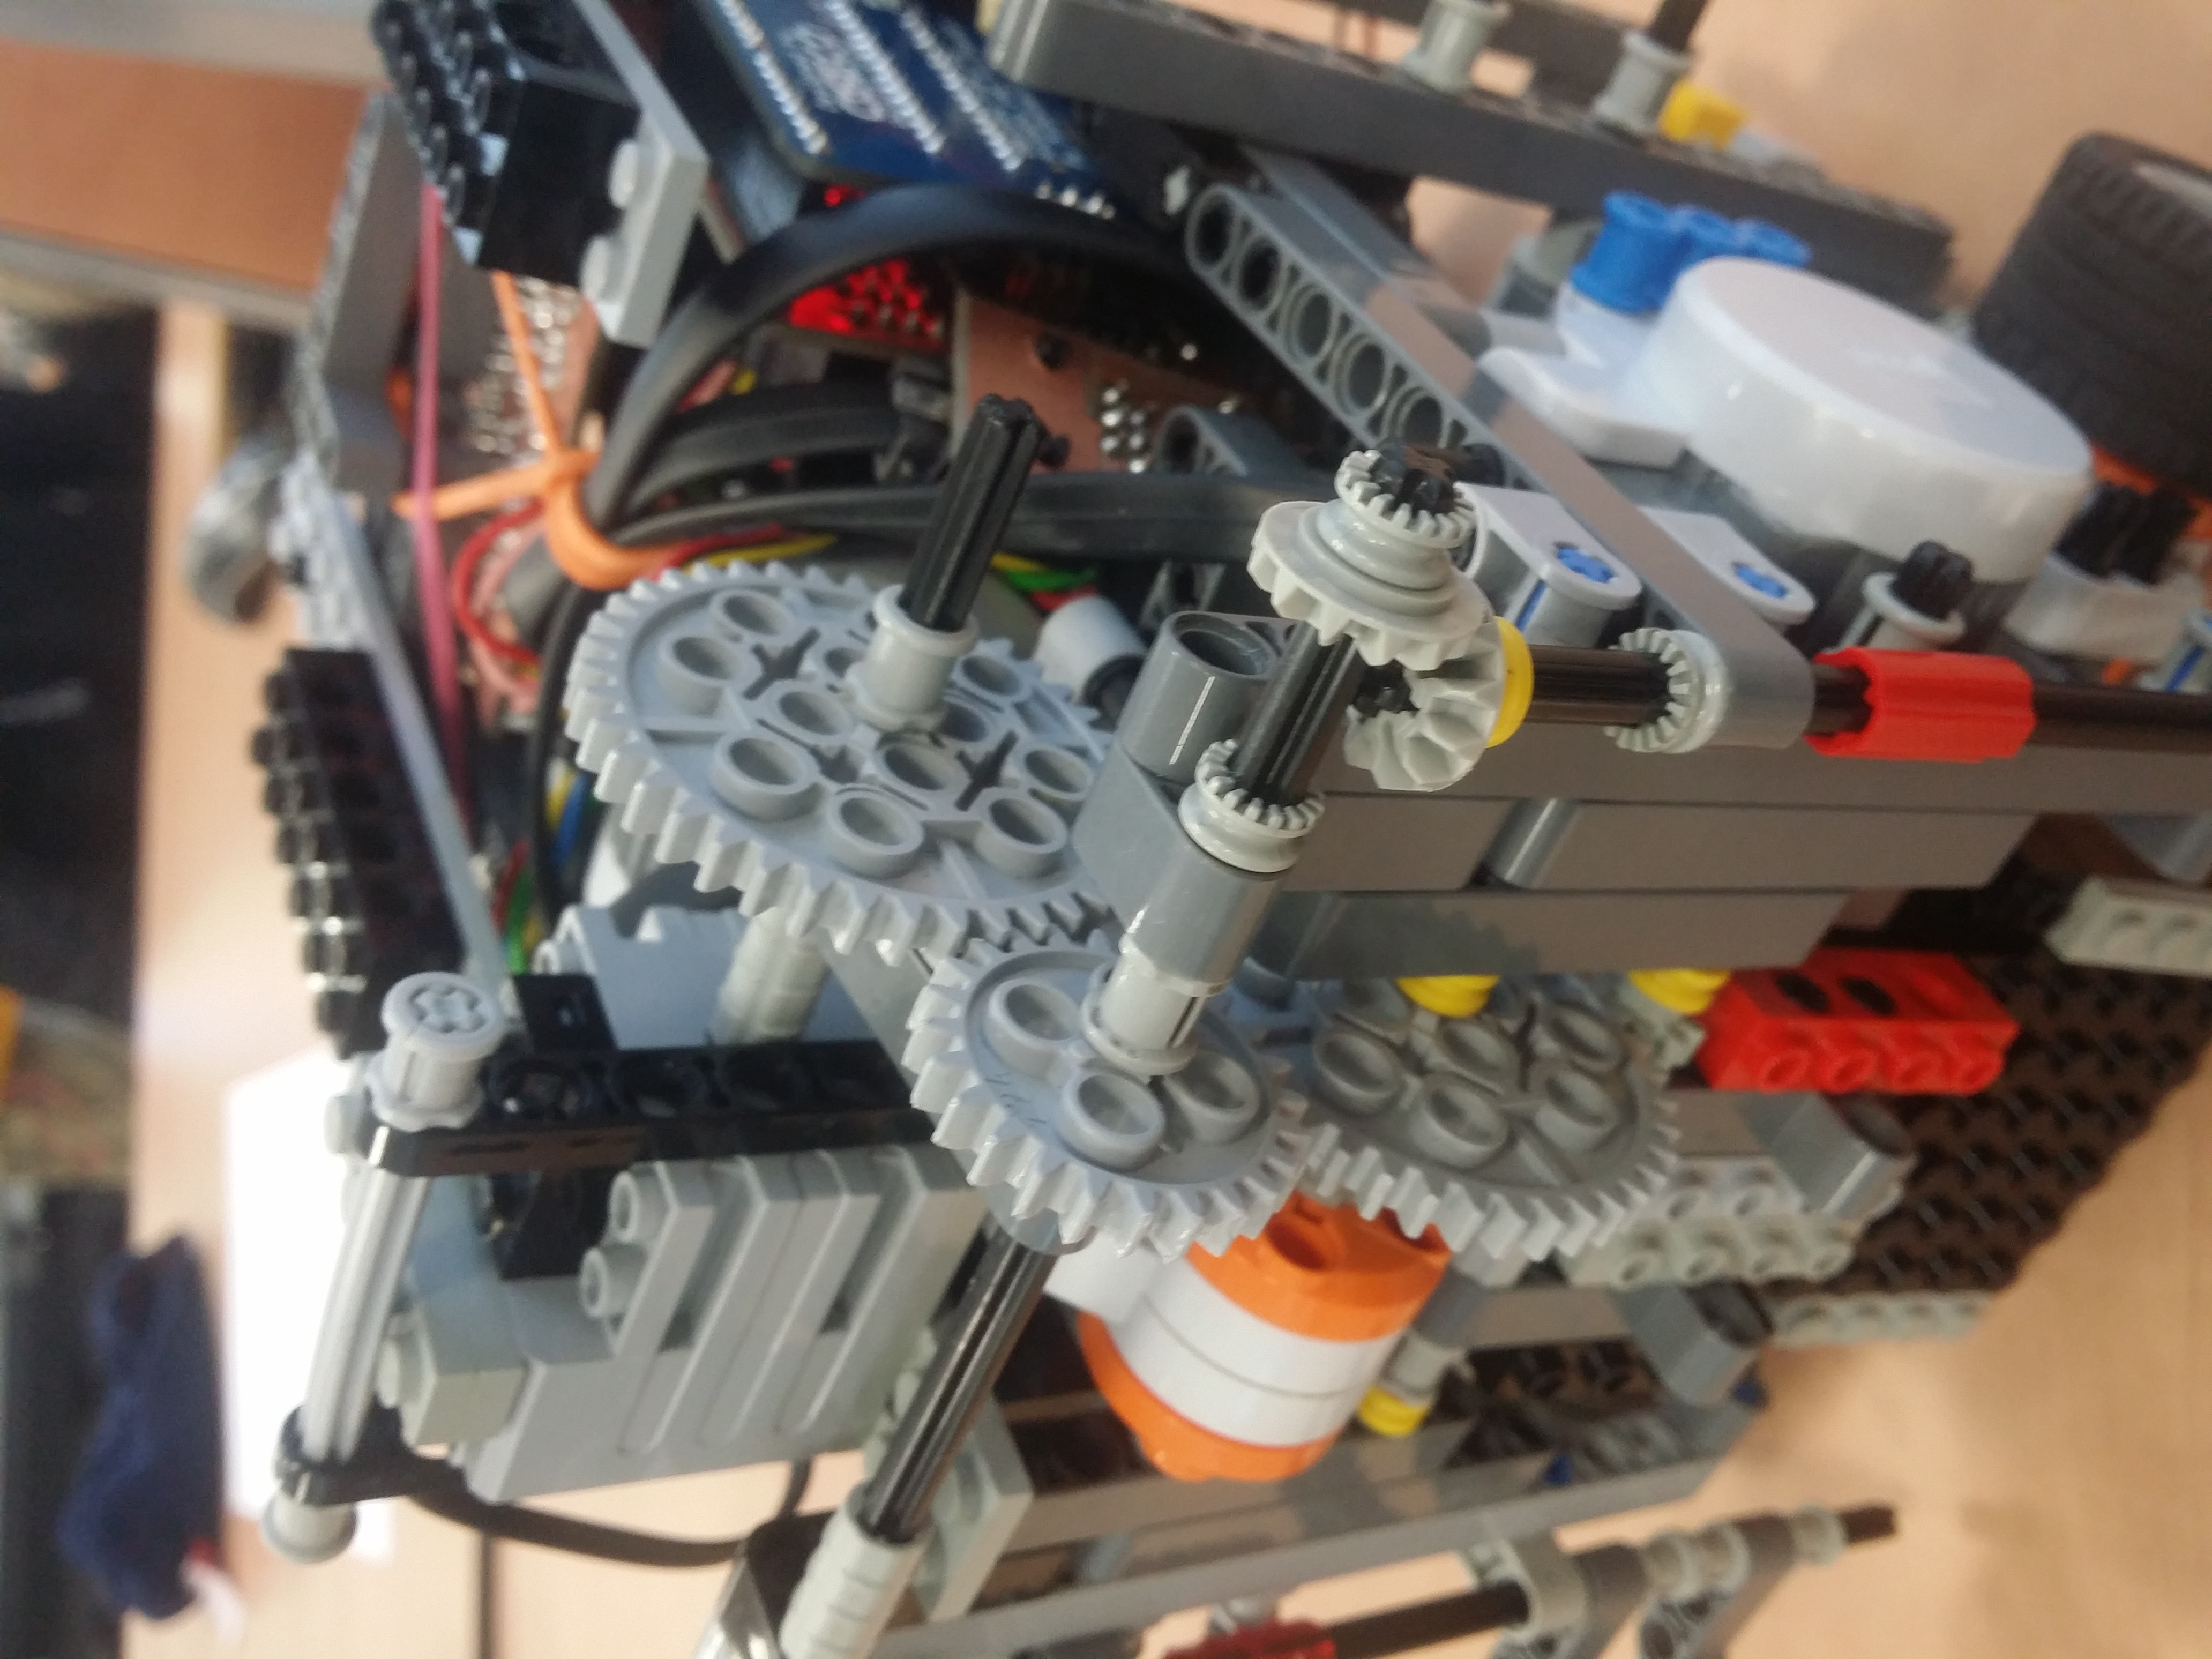
\includegraphics[scale=.065,angle=-90]{gears.jpg}
		\caption{Gears for the grabber}
		\label{fig:gears}
	\end{minipage}
	
\end{figure}


\section{Hardware components}

\subsection{Wheels}
Could you be more descriptive? i.e. why you decided to build it like that ? Why mixture of wheel types ? How the robot can turn? what kind of problems you were trying to omit ? It is a far to short and vague description.  Since your robot has four holonomic wheels now, could you describe why it is a four-wheeled robot now? What is the main feature, advantage of the holonomic property? What is exactly this property.  What are NXT motors ? how they work?


The current design has four holonomic wheels, which allows Venus to move in any direction. All wheels are powered by NXT motors.

\subsection{Kicker}
Even though the idea of the kicker that uses elastics was appealing as this made
the kick more powerful, it was almost impossible to predict the distance the
ball will travel. Because of that the newer design had a
kicker that was powered by an NXT motor with gears. The kicker operated by going backwards inside the robot from the starting low position as seen in Figures \ref{fig:kicker}-\ref{fig:kicker_back} and then kicked
forwards and touched the ball.
\begin{figure}[ht]
	\centering
	\begin{minipage}[b]{.3\textwidth}
        \centering
		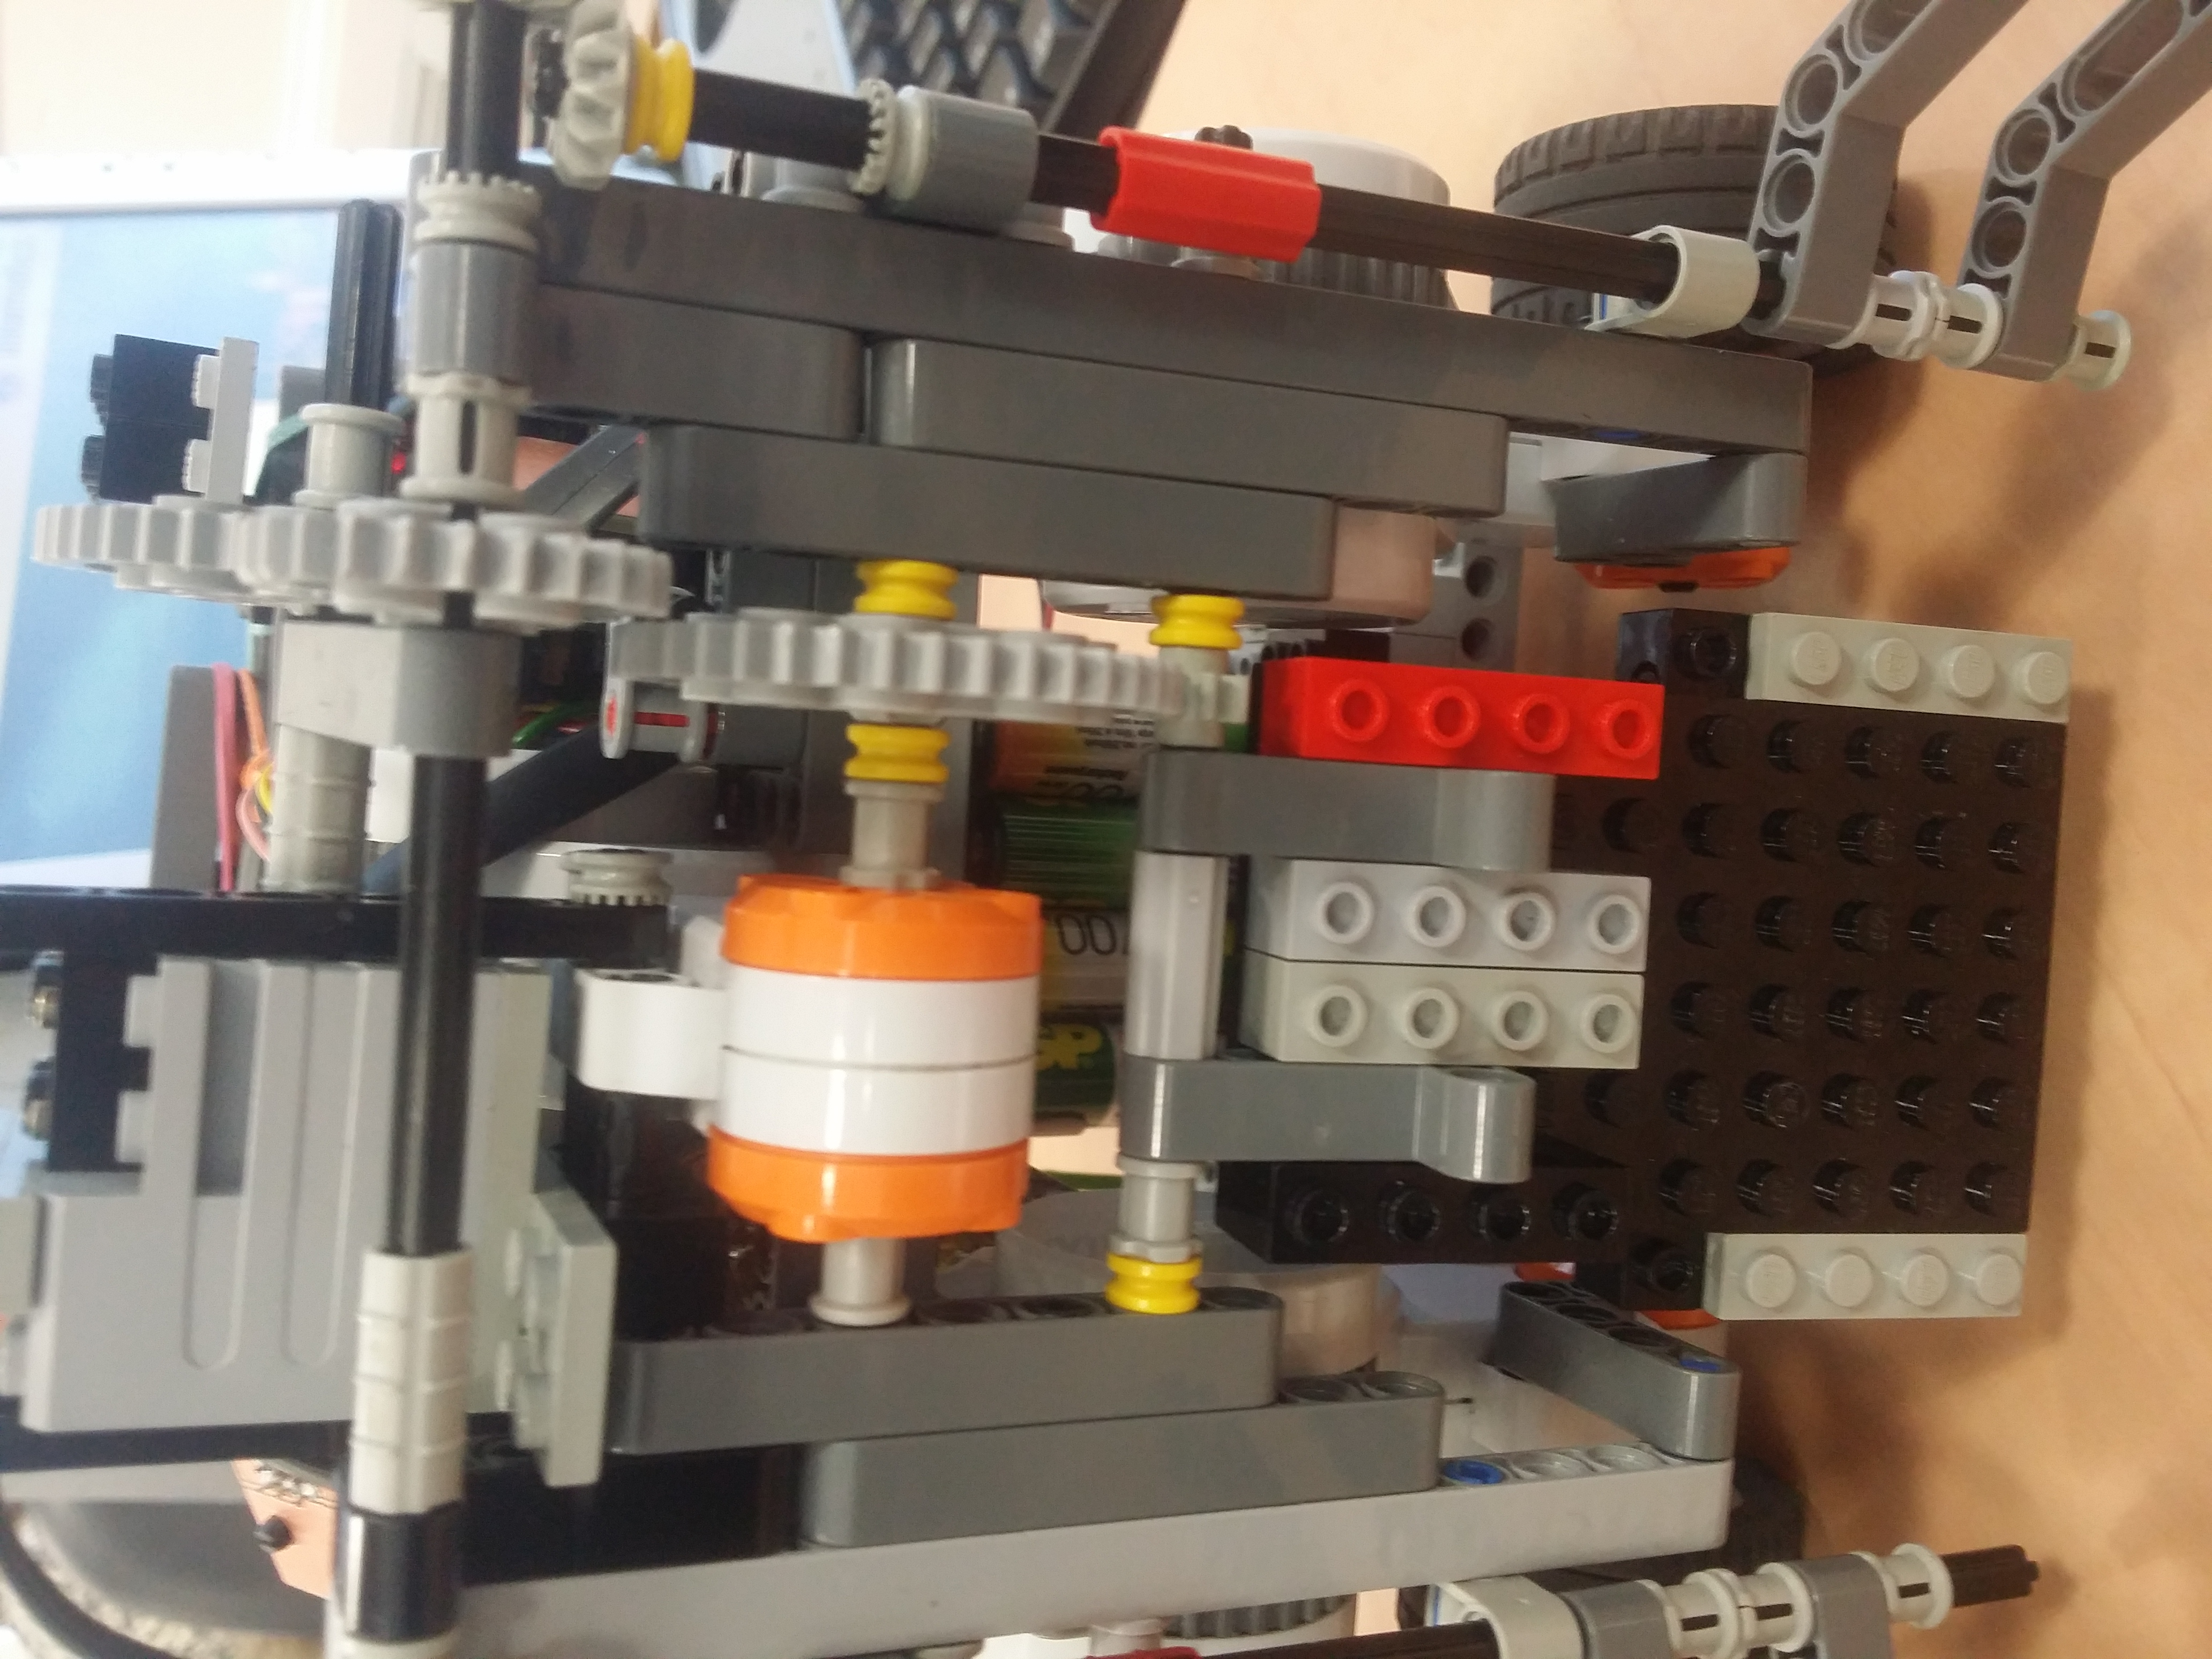
\includegraphics[scale=0.04, angle=-90]{kick_front.jpg}
		\caption{Kicker in still position}
		\label{fig:kicker}
	\end{minipage}
	~
	\begin{minipage}[b]{.3\textwidth}
        \centering
		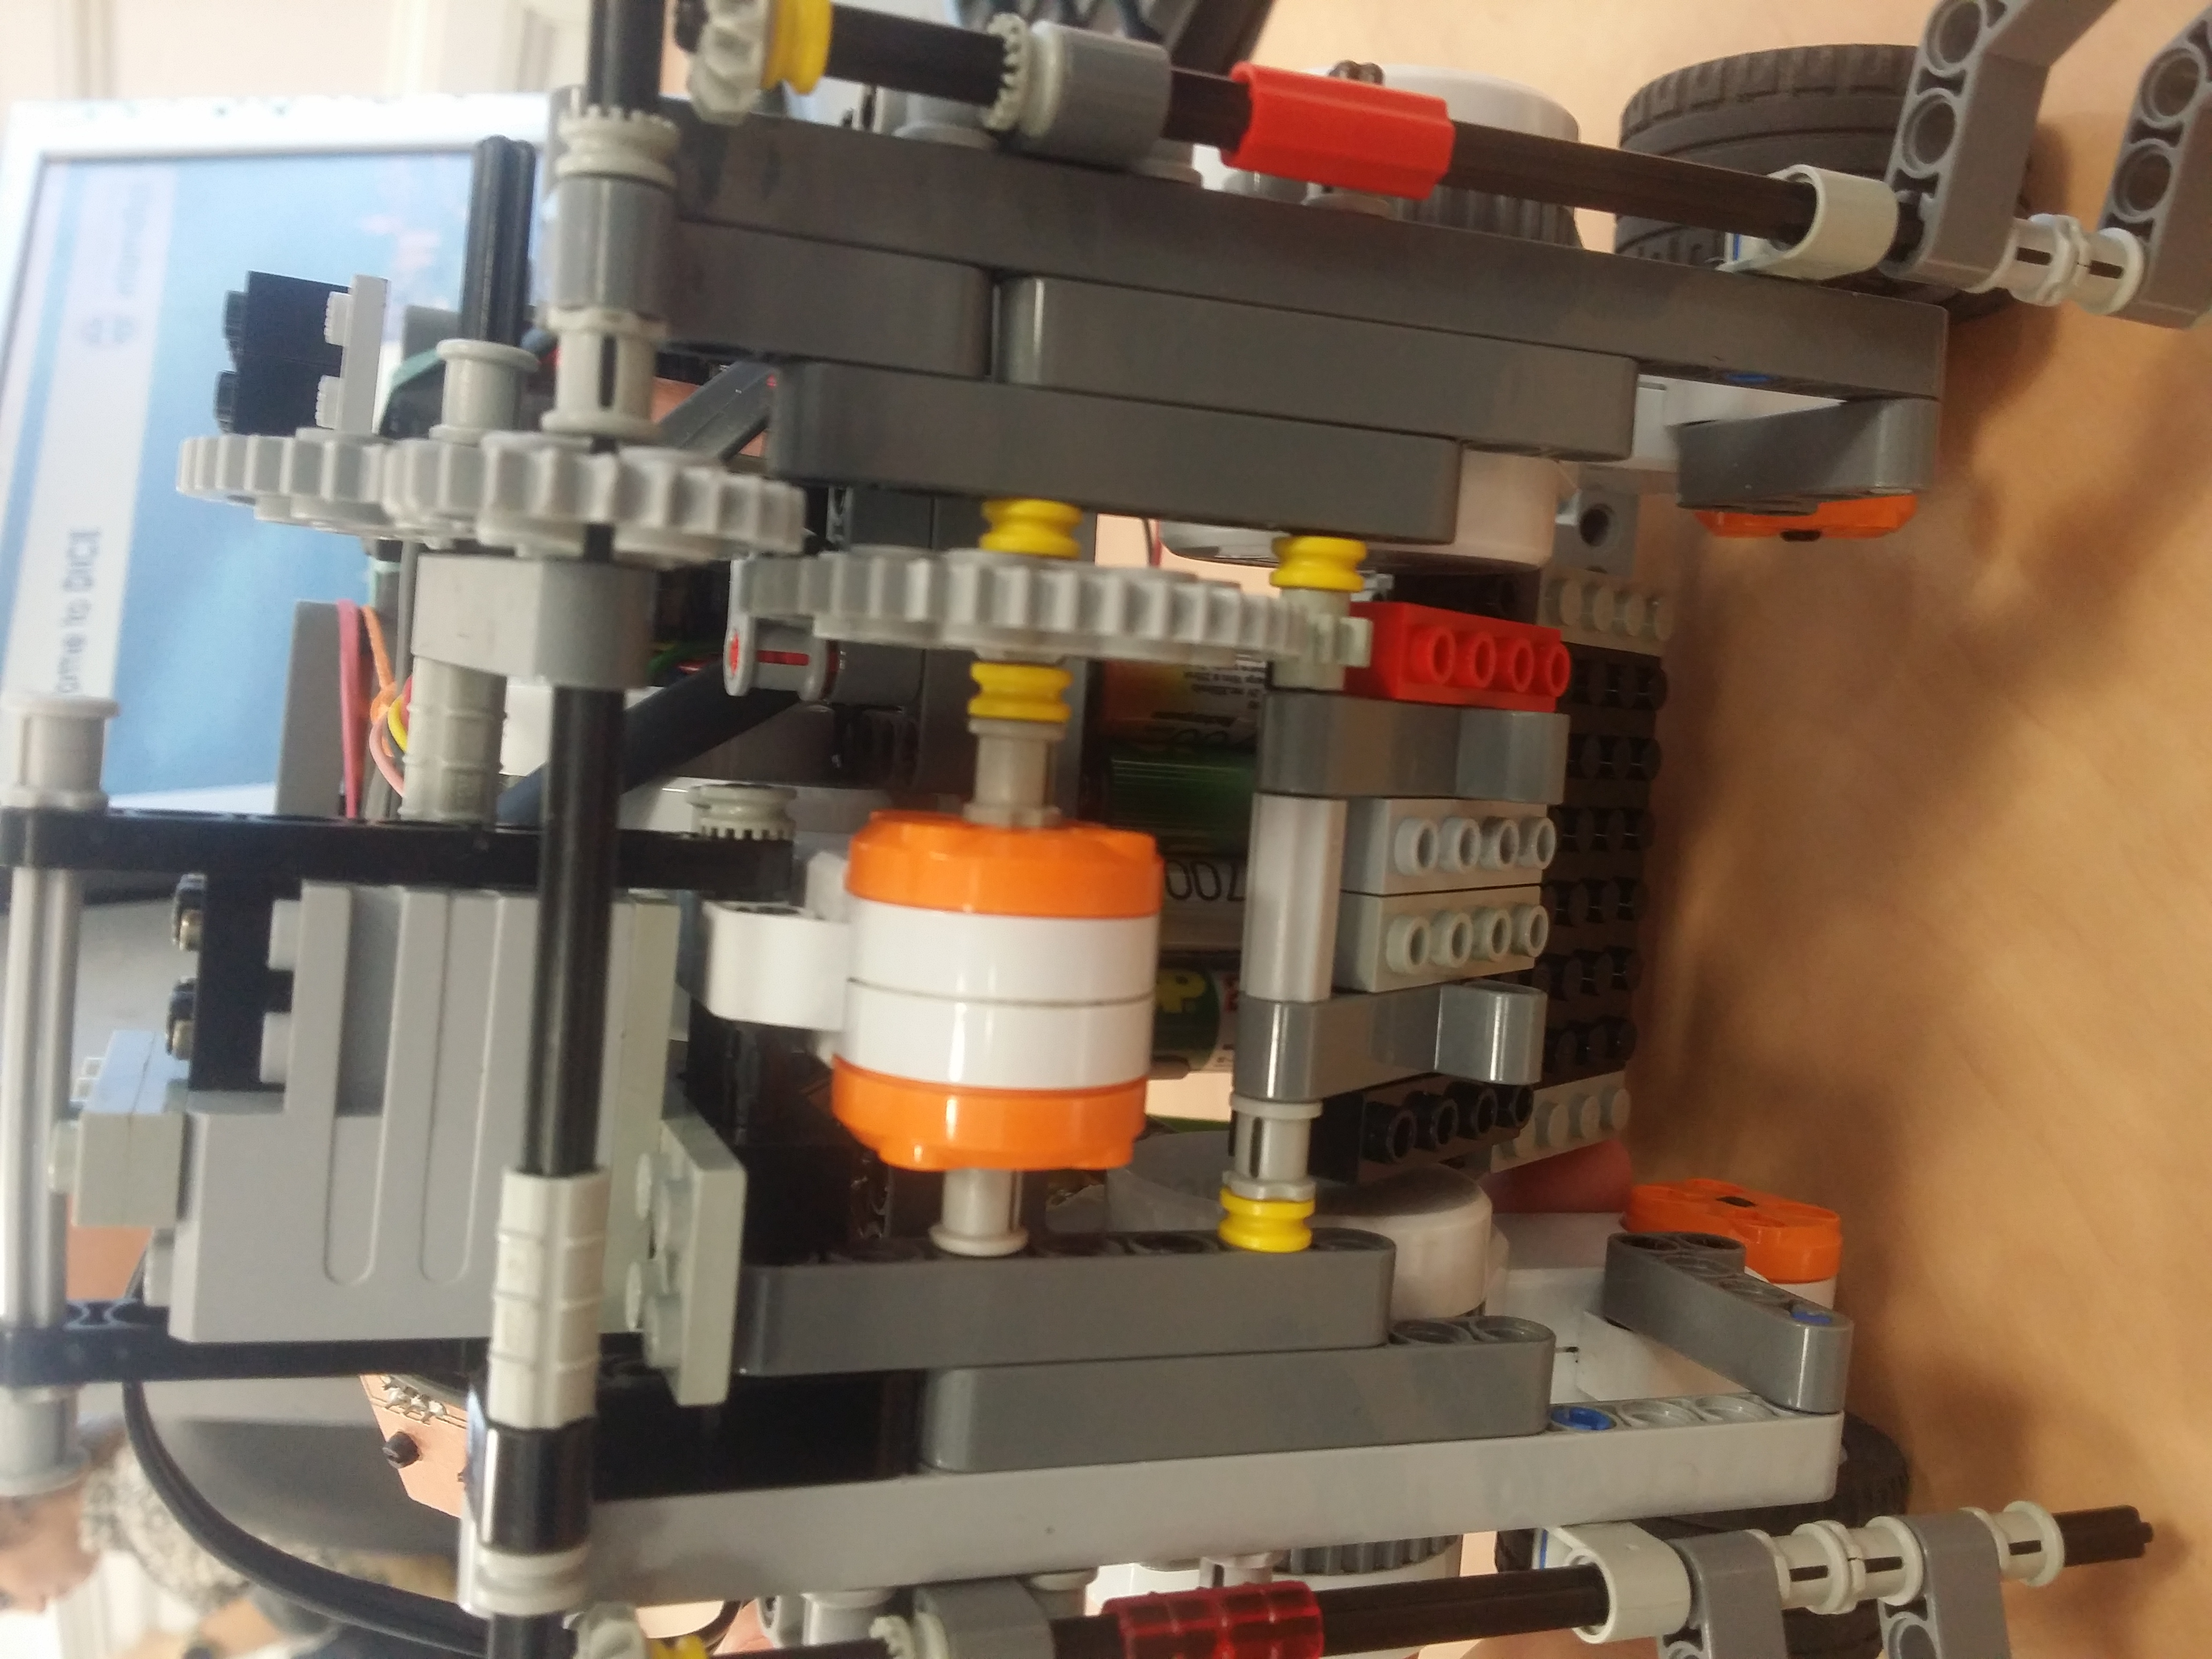
\includegraphics[scale=0.04, angle=-90]{kick_middle.jpg}
		\caption{Kicker starts going back}
		
	\end{minipage}
	~
	\begin{minipage}[b]{.3\textwidth}
        \centering
		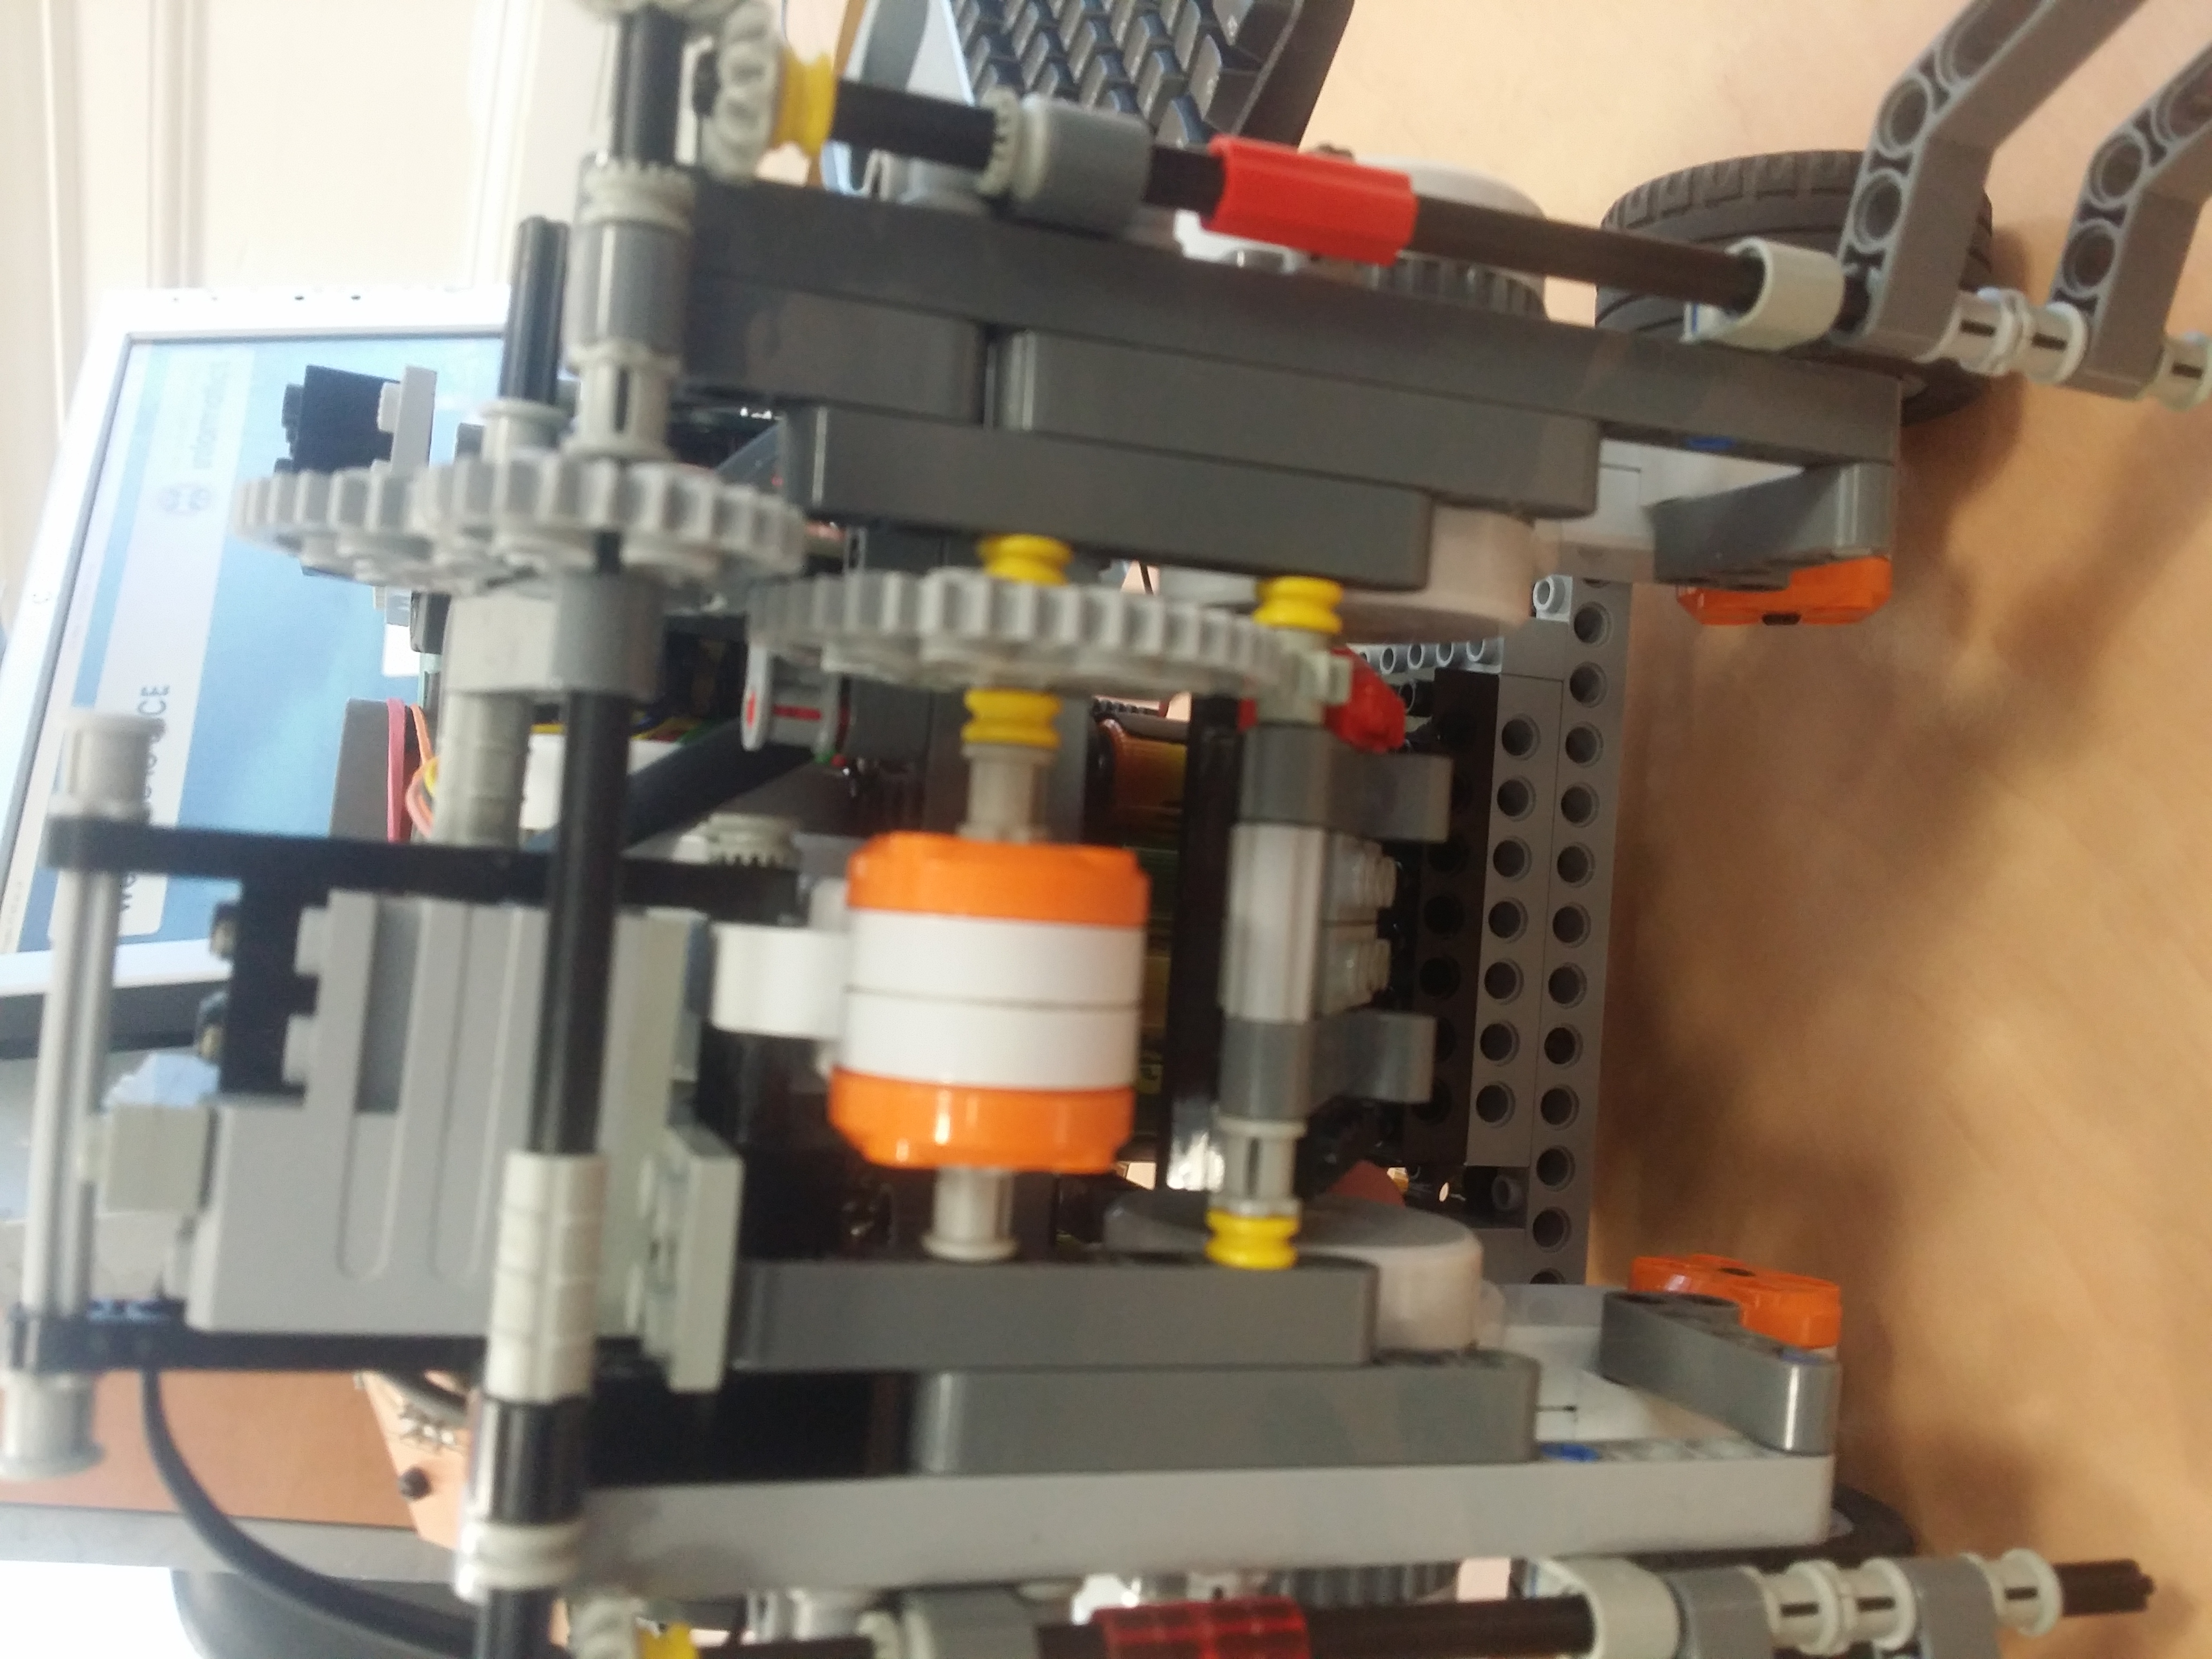
\includegraphics[scale=0.04, angle=-90]{kick_back.jpg}
		\caption{Kicker in the back position}
		\label{fig:kicker_back}
	\end{minipage}
	
\end{figure}

Our newest design doesn't have a kicker. The kick is made by turning  the robot and opening the grabber at the same time. This creates a momentum necessary to make a kick (Figure \ref{fig:kick_action}). 
\begin{figure}
    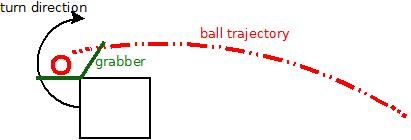
\includegraphics[scale=.7]{kick}
    \caption{High level diagram of how the kick is performed}
    \label{fig:kick_action}
\end{figure}


\subsection{Grabber}
The grabber for the previous design consisted of two symmetric parts placed one a bit above the other and was placed on the sides of the front part of the robot (Figure \ref{fig:gears}). They interlocked when the robot needs to catch the ball and we also kept them in a closed position during movements without the ball. We opened the grabber only before catching. This ensured that the grabber don't get broken against other robots or walls. We have used two bevel gears in order to be able to move grabbers with motor being on top of the robot. The current design of the grabber doesn't differ much and can be seen in Figure FIGURE. The grabber is powered by a single Electric Technic Mini-Motor 9v with gears.

\section{Documentation of the code}

\begin{figure}[ht!]
\centering
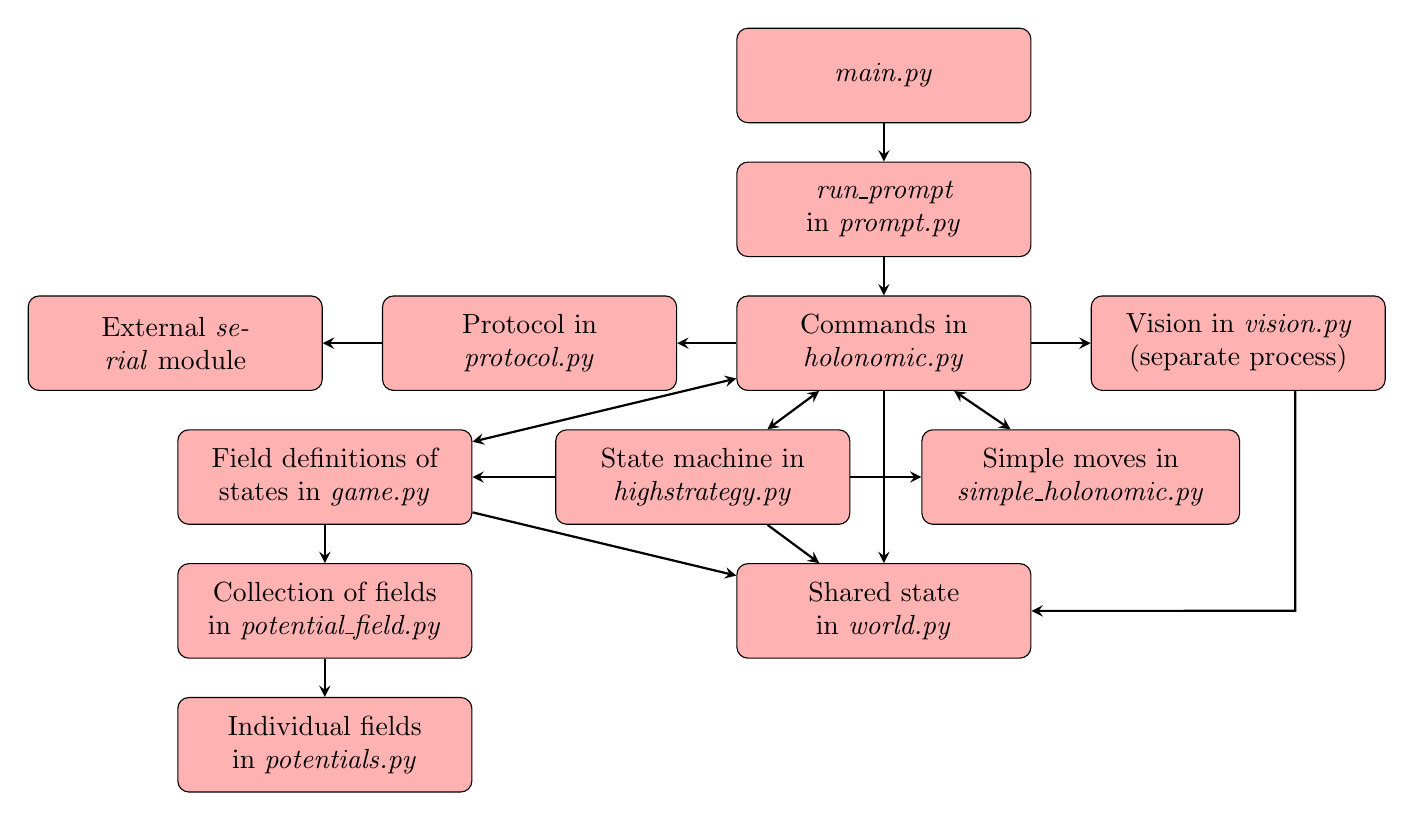
\begin{tikzpicture}[node distance=1.7cm]

\node (main) [module] {\textit{main.py}};
\node (prompt) [module, below of=main] {\textit{run\_prompt} in \textit{prompt.py}};
\draw [arrow] (main) -- (prompt);
\node (commands) [module, below of=prompt] {Commands in \textit{holonomic.py}};
\draw [arrow] (prompt) -- (commands);
\node (protocol) [module, left of=commands, xshift=-2.8cm] {Protocol in \textit{protocol.py}};
\draw [arrow] (commands) -- (protocol);
\node (serial) [module, left of=protocol, xshift=-2.8cm] {External \textit{serial} module};
\draw [arrow] (protocol) -- (serial);

\node (world) [module, below of=commands, yshift=-1.7cm] {Shared state in \textit{world.py}};
\draw [arrow] (commands) -- (world);

\node (vision) [module, right of=commands, xshift=2.8cm] {Vision in \textit{vision.py} (separate process)};
\draw [arrow] (commands) -- (vision);
\draw [arrow] (vision.320) |- ++(0, -2.792cm) -- (world);

\node (moves) [module, below of=commands, xshift=2.5cm, text width=3.8cm] {Simple moves in \textit{simple\_holonomic.py}};
\draw [arrow, <->] (commands) -- (moves);

\node (state) [module, below of=commands, xshift=-2.3cm] {State machine in \textit{highstrategy.py}};
\draw [arrow, <->] (commands) -- (state);
\draw [arrow] (state) -- (moves);
\draw [arrow] (state) -- (world);

\node (game) [module, below of=commands, xshift=-7.1cm] {Field definitions of states in \textit{game.py}};
\draw [arrow, <->] (commands) -- (game);
\draw [arrow] (state) -- (game);
\draw [arrow] (game) -- (world);
\node (field) [module, below of=game] {Collection of fields in \textit{potential\_field.py}};
\draw [arrow] (game) -- (field);
\node (pot) [module, below of=field] {Individual fields in \textit{potentials.py}};
\draw [arrow] (field) -- (pot);

\end{tikzpicture}
\caption{Dependency graph of Python modules in the system}
\label{fig:overview}
\end{figure}

The code is subdivided into several Python modules as seen in Figure \ref{fig:overview}. The module \textit{main} is used to launch the \textit{prompt} module. The commands in the prompt are provided by the \textit{commands} module. It creates instances of protocol, vision, and state machine objects from the respective modules. The vision object is run on a separate thread to process frames asynchronously with constantly updated shared world state kept in a \textit{World} object. At the same time the prompt is provided for the user. The command to run the strategy is called \texttt{hs}. This command constantly queries the state machine in the \textit{highstrategy} module. The state machine checks the world state to decide which state it is currently in and then performs the associated action. It is done either by handing over the execution to \textit{game} module to construct a potential field and perform the best action based on it or performing a predefined move from the \textit{simple\_holonomic} module.

All code except the colour calibration user interface in the \textit{vision} module is an original work. Libraries used are \textit{pyserial}, \textit{numpy}, \textit{scipy}, and \textit{OpenCV}.

\subsection{Communications}

The communication interface between the Arduino and PC is low level as the PC decides and specifies the individual motor numbers and rotary encoder value or time duration for which they will be powered. Then the Arduino sends acknowledgement to the PC about the arrival of the command, turns the motors on, and sets the specified timeouts to stop them. The messages are human-readable, newline-terminated and tokens inside them are separated by spaces. The specified motor power can be negative, in which case it means backwards direction. Each message which changes the state of the robot has a sequence number and checksum that are checked in the Arduino. The messages used in the protocol are listed in Table \ref{tab:messages}. The communication messages are constructed in the \textit{Protocol} class using methods named after the corresponding message in \texttt{control/protocol.py} and these are used in the motion commands in \texttt{control/holonomic.py}.

\begin{table}[h!]
\centering
\begin{tabular}{ | l | l | }
    \hline
    Rotate the motors for $n$ ms &
    \small{\texttt{M seqNo checksum n motorNo power...}} \\ \hline
    Rotate the motors for $n$ rotary values &
    \small{\texttt{R seqNo checksum n motorNo power...}} \\ \hline
    Rotate the motors indefinitely &
    \small{\texttt{V seqNo checksum motorNo power...}} \\ \hline
    Stop all motors &
    \small{\texttt{S seqNo checksum}} \\ \hline
    Return \texttt{D} if all motors are stopped &
    \small{\texttt{I}} \\ \hline
    Handshake, reset the sequence number &
    \small{\texttt{H}} \\ \hline
    Query light sensor, return \texttt{D} or \texttt{N} &
    \small{\texttt{A threshold}} \\ \hline
    Transfer a byte to I2C bus &
    \small{\texttt{T byteInDecimalASCII}} \\ \hline
\end{tabular}
\caption{Messages available in the protocol}
\label{tab:messages}
\end{table}

\subsection{Arduino}

\begin{figure}[ht!]
\centering
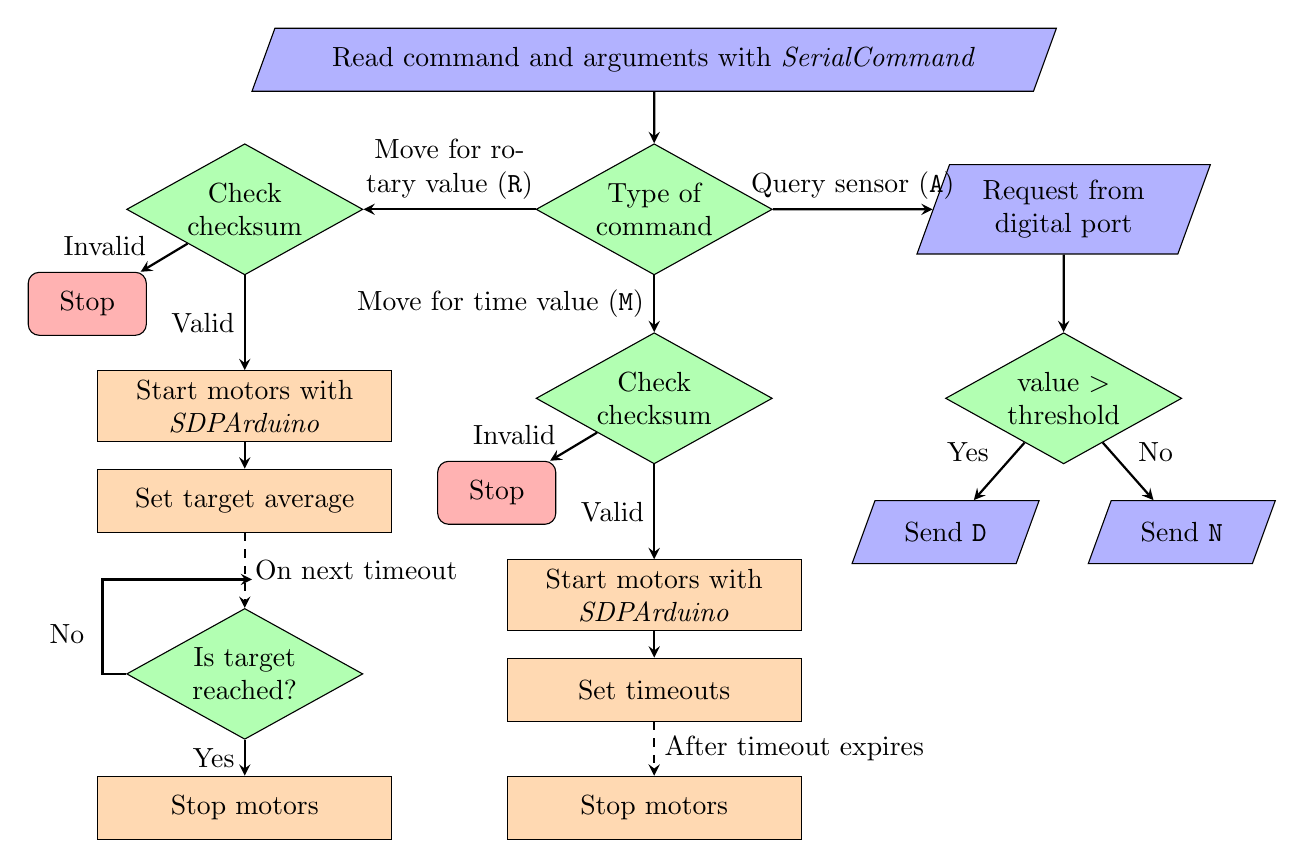
\begin{tikzpicture}[node distance=1.2cm]

\node (inCmd) [io] {Read command and arguments with \textit{SerialCommand}};
\node (decType) [decision, below of=inCmd, yshift=-.7cm] {Type of command};
\draw [arrow] (inCmd) -- (decType);

\node (decCheck1) [decision, left of=decType, xshift=-4cm] {Check checksum};
\draw [arrow] (decType) -- node [anchor=south, text width=3cm, text centered] {Move for rotary value (\texttt{R})} (decCheck1);
\node (stop1) [startstop, below of=decCheck1, xshift=-2cm] {Stop};
\draw [arrow] (decCheck1) -- node [anchor=south east, yshift=-.1cm, xshift=-.1cm] {Invalid} (stop1);
\node (motors1) [process, below of=decCheck1, yshift=-1.3cm, text width=3.5cm] {Start motors with \textit{SDPArduino}};
\draw [arrow] (decCheck1) -- node [anchor=east] {Valid} (motors1);
\node (target) [process, below of=motors1] {Set target average};
\draw [arrow] (motors1) -- (target);
\node (decTarget) [decision, below of=target, yshift=-1cm] {Is target reached?};
\draw [arrow, dashed] (target) -- node [anchor=west] {On next timeout} (decTarget);
\draw [arrow] (decTarget.west) |- node [anchor=east, xshift=-.4cm, yshift=.5cm] {No} ++(-.3cm, 0)
                               |- ++(0, 1.2cm)
                               -- ++(1.9cm, 0);
\node (stopMotors1) [process, below of=decTarget, yshift=-.5cm] {Stop motors};
\draw [arrow] (decTarget) -- node [anchor=east] {Yes} (stopMotors1);


\node (decCheck2) [decision, below of=decType, yshift=-1.2cm] {Check checksum};
\draw [arrow] (decType) -- node [anchor=east] {Move for time value (\texttt{M})} (decCheck2);
\node (stop2) [startstop, below of=decCheck2, xshift=-2cm] {Stop};
\draw [arrow] (decCheck2) -- node [anchor=south east, yshift=-.1cm, xshift=-.1cm] {Invalid} (stop2);
\node (motors2) [process, below of=decCheck2, yshift=-1.3cm, text width=3.5cm] {Start motors with \textit{SDPArduino}};
\draw [arrow] (decCheck2) -- node [anchor=east] {Valid} (motors2);
\node (timeouts) [process, below of=motors2] {Set timeouts};
\draw [arrow] (motors2) -- (timeouts);
\node (stopMotors2) [process, below of=timeouts, yshift=-.3cm] {Stop motors};
\draw [arrow, dashed] (timeouts) -- node [anchor=west] {After timeout expires} (stopMotors2);

\node (req) [io, right of=decType, xshift=4cm, text width=2.5cm] {Request from digital port};
\draw [arrow] (decType) -- node [anchor=south, text width=3cm, text centered] {Query sensor (\texttt{A})} (req);
\node (decComp) [decision, below of=req, yshift=-1.2cm] {value $>$ threshold};
\draw [arrow] (req) -- (decComp);
\node (sendD) [io, below of=decComp, xshift=-1.5cm, yshift=-.5cm] {Send \texttt{D}};
\draw [arrow] (decComp) -- node [anchor=south east] {Yes} (sendD);
\node (sendN) [io, below of=decComp, xshift=1.5cm, yshift=-.5cm] {Send \texttt{N}};
\draw [arrow] (decComp) -- node [anchor=south west] {No} (sendN);

\end{tikzpicture}
\caption{Flowchart of message processing in the Arduino}
\label{fig:flow}
\end{figure}

The Arduino code uses the \textit{SerialCommand} library to buffer and tokenize the commands received over the serial link. Messages changing the world state are sent with a sequence number and checksum which is the sum of all the parameters following it. If the sequence number matches the one from the last command, acknowledgement is sent but no further work is performed for the duplicate message. This handles the situation arising when an acknowledgement from the Arduino does not reach the PC and and the PC generates a duplicate message. If the checksum does not match, the Arduino code ignores the message and does not send an acknowledgement, thus forcing the PC to send the same message again.

If any of the motor move commands are sent, the motors are started immediately using the \textit{SDPArduino} library. Then the Arduino schedules when to stop the motors and there are two methods to perform that: either a time value or rotary encoder value. The flowchart for these two methods, along with querying the light sensor, are detailed in Figure \ref{fig:flow}.
In the case of the time value, a timeout is set to stop each single motor using
\textit{setTimeout} from the \textit{SimpleTimer} library.
In the case of rotary encoder value, \textit{setInterval} is used which calls
a function every 5 ms that queries the rotary encoder board and stops the motors
when the average of all four motor rotary encoder values reaches the target value. These approaches using timers
allows the robot to receive commands asynchronously, that is, a command is not
blocking during its execution and the PC software could, for example, send another command simultaneously to engage the kicker while the robot is in motion.
The Arduino message handling is located in \texttt{arduino/arduino.ino} file.

A buffer of upcoming motor jobs has also been implemented in the Arduino code to ensure continuous motion but it was deemed unnecessary as vision could issue new commands quickly enough without the robot coming to halt. The current implementation also never stops a motor when a new command arrives for the same motor, instead it just executes the new command, ensuring continuous motion.

\subsection{Vision}

In our opinion, the vision is our unique feature of this project. We have built the whole system from scratch without borrowing any code from previous years. This allowed us to implement things we might not have been able to do with an existing system. 
\\In order to be able to detect robots and the ball, we go through the following steps:

\begin{enumerate}
\item For the relevant room (0 or 1) read files containing the following data: brightness, contrast,     saturation, hue values (room0.txt), minimum and maximum HSV values for each color that we want to detect (color0.txt), distortion (dist0.txt). 
\item The image from the video feed is blurred (using \textit{cv2.GaussianBlur}) and the mask is created (there is a possibility of calibration if some colors are not detected well enough).
\item We draw circles of relevant colors that are in the mask except red (the ball).
\item Find the ball.
\item Find robots.
\end{enumerate}

\subsubsection{Calibration}
When the video feed is opened, there are bars on the top that allow you to adjust brightness, hue, saturation and contrast. There is also a bar that is called 'calibration', which takes boolean values 0 or 
1. If you want to calibrate, you just need to move this bar to the right. 
\\When calibration mode is chosen another frame is opened, (it is a picture of the pitch captured when you entered this mode). In the top left corner, there is a ball representing the color that is currently being calibrated. In order to calibrate, you need to click on the pixels of this color. If the values that are read when you click do not match those expected for this color, they are discarded. With each new click a HSV values are stored, when calibration is finished, the range of all clicks is calculated for each color. This means you need to click multiple times in order to get a better result. This range is then stored to a file color0.txt overwriting anything else that was there before. We have minimum and maximum values for all colors except red, which has four values, because of the HSV cone. 
\\If you want to switch color, press 'q'. After all colors are done, the calibration mode is exited automatically. 

\subsubsection{Finding the robots}
Once we have detected all the colors, we try to decide where the actual robots are. In order to do that we need all robots to be on the pitch in the beginning when we run the code. 
\\There is a list of four robots we need to detect. We sort all colors we detected by their size (from biggest to lowest). Then for each robot, we check the following:

\begin{enumerate}
\item If we see all the colors on approximately right distances (given in rules) from each other, it is a perfect case and we say we have detected the robot.
\item If we can see the centre and the spot that is in bottom left corner (the one that differs from others), then we know the centre of mass, and we draw an orientation vector by rotating the line between centre and the spot we detected.
\item If we only can detect a centre spot, then we draw an orientation vector that we have seen in previous frame.
\item If there are three spots of the same color, then the centre of mass is calculated by taking the centre of two furthest from each other points. It is not exact, but gives a good approximation. The orientation vector is then drawed through the centre of mass and the middle point of two front spots.
\end{enumerate}
This ensures that we are able to detect robots even if at some point we cannot detect all the colors. Apart from the above steps, we also check that the centre of mass is on the reasonable distance from where it was in the last frame (to avoid robots flipping). Furthermore, if we have found the robot of one type (say our teammate), then we restrict it from finding another one. 
\\When the robots are found we draw a box around them (green for Venus and yellow for teammate red for opposite team) and label with a number from 0 to 3, where 0 is Venus, 1 is our teammate and 3,4 are opposite team robots. 

\subsubsection{Finding the ball}

We restrict the number of circles of each color we want to detect, e.g. 2 blue, 2 yellow, 8 green etc. For red, it is 9, because we are likely to think that pink is red. If at any point we are not able to see any red spots, we decide that the ball is underneath one of the robots or not on the pitch. If we can see the spot that is not part of the robots detected earlier, we store ball's position as a stack that has centres of mass of the ball for the last 6 frames (every time new value comes in, last one is popped). We check the first and the last values in this stack. If their difference is more than 10 pixels, then the ball is moving and we draw its trajectory.  

\subsection{Strategy}

table with all states

\section{Sensors}
\subsection{Rotary encoder board}

Each NXT motor is connected to the rotary encoder board which is depicted in Figure \ref{fig:rotary}. The connections in the anticlockwise order from the top are: the I2C bus to the Arduino, back right motor, back left motor, front left motor, and front right motor. Using this board the information about the amount of rotations the motor has performed since the last query is available for the Arduino code as a separate integer for every motor. Every 5 ms the board is queried whether the target value has been reached. After the average of the rotary values of all four motors becomes greater or equal to the target value, the motors are stopped.

\begin{figure}[ht!]
\centering
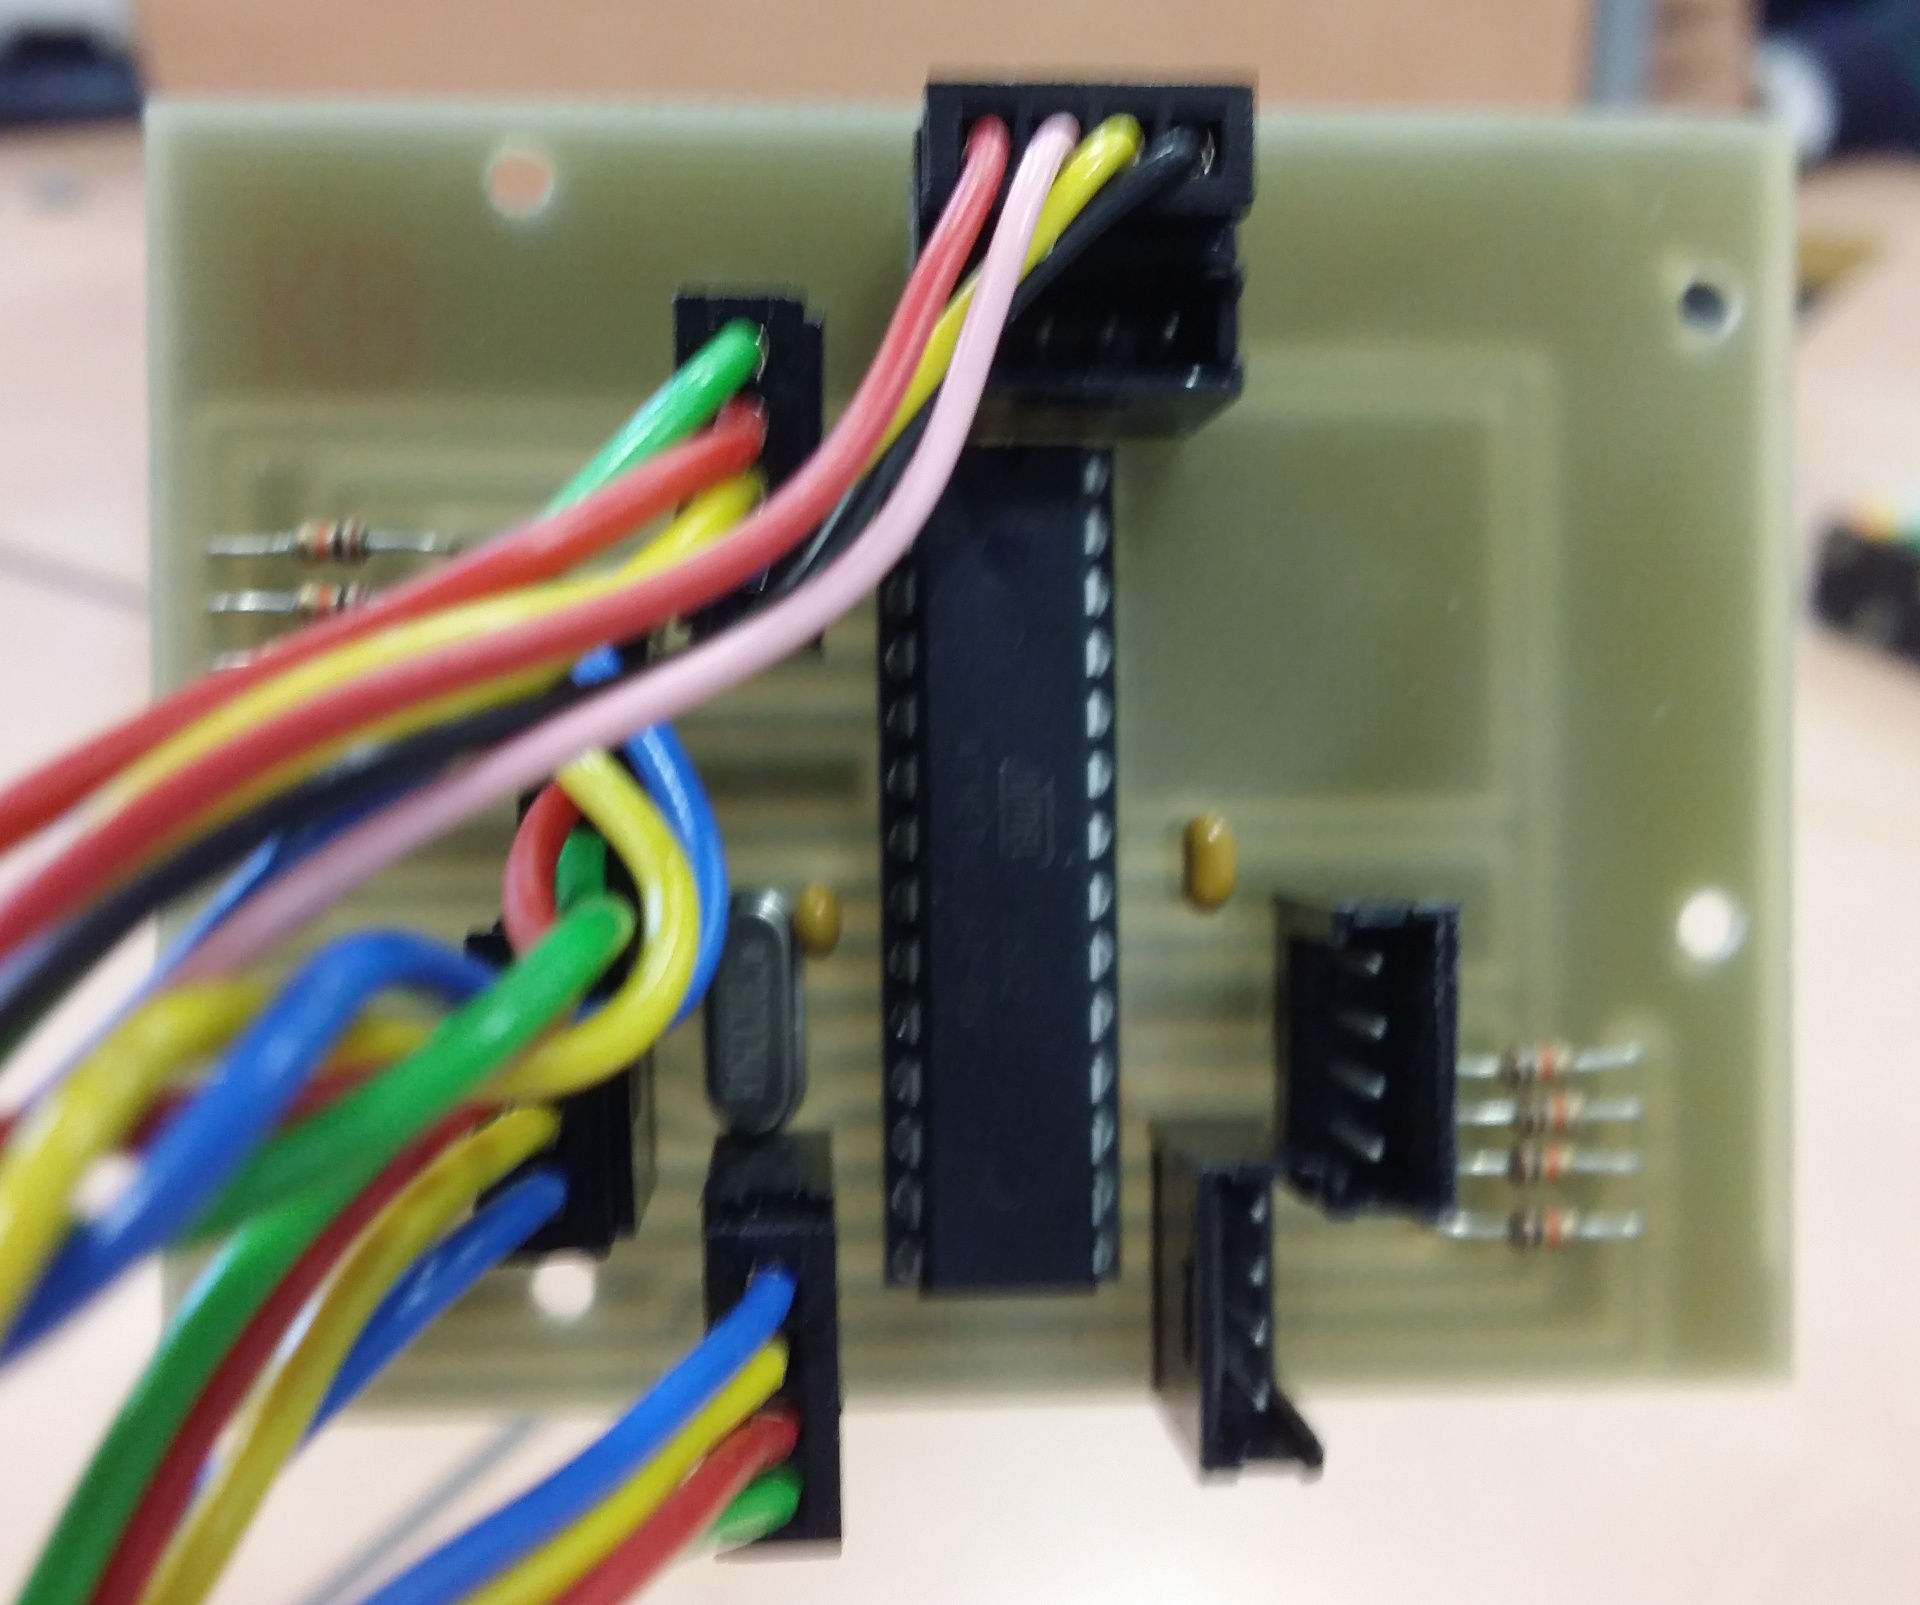
\includegraphics[scale=.1]{rotary1}
\caption{The rotary encoder board}
\label{fig:rotary}
\end{figure}

\subsection{Light sensor}

The light sensor is located above the grabber as seen in Figure \ref{fig:sensor}. It is used to check whether
the robot has successfully acquired the ball after grabbing. The sensor
provides an integer value that increases the greater the distance to the
nearest object in its direct line of sight is. Then the Arduino compares the integer
to a predefined threshold corresponding to the red ball. Sometimes a white
line inside the pitch can be mistaken for the ball due to their similar sensor
values. An IR sensor was also tested and its returned values were deemed less reliable than
those of the light sensor.

\begin{figure}[ht!]
\centering
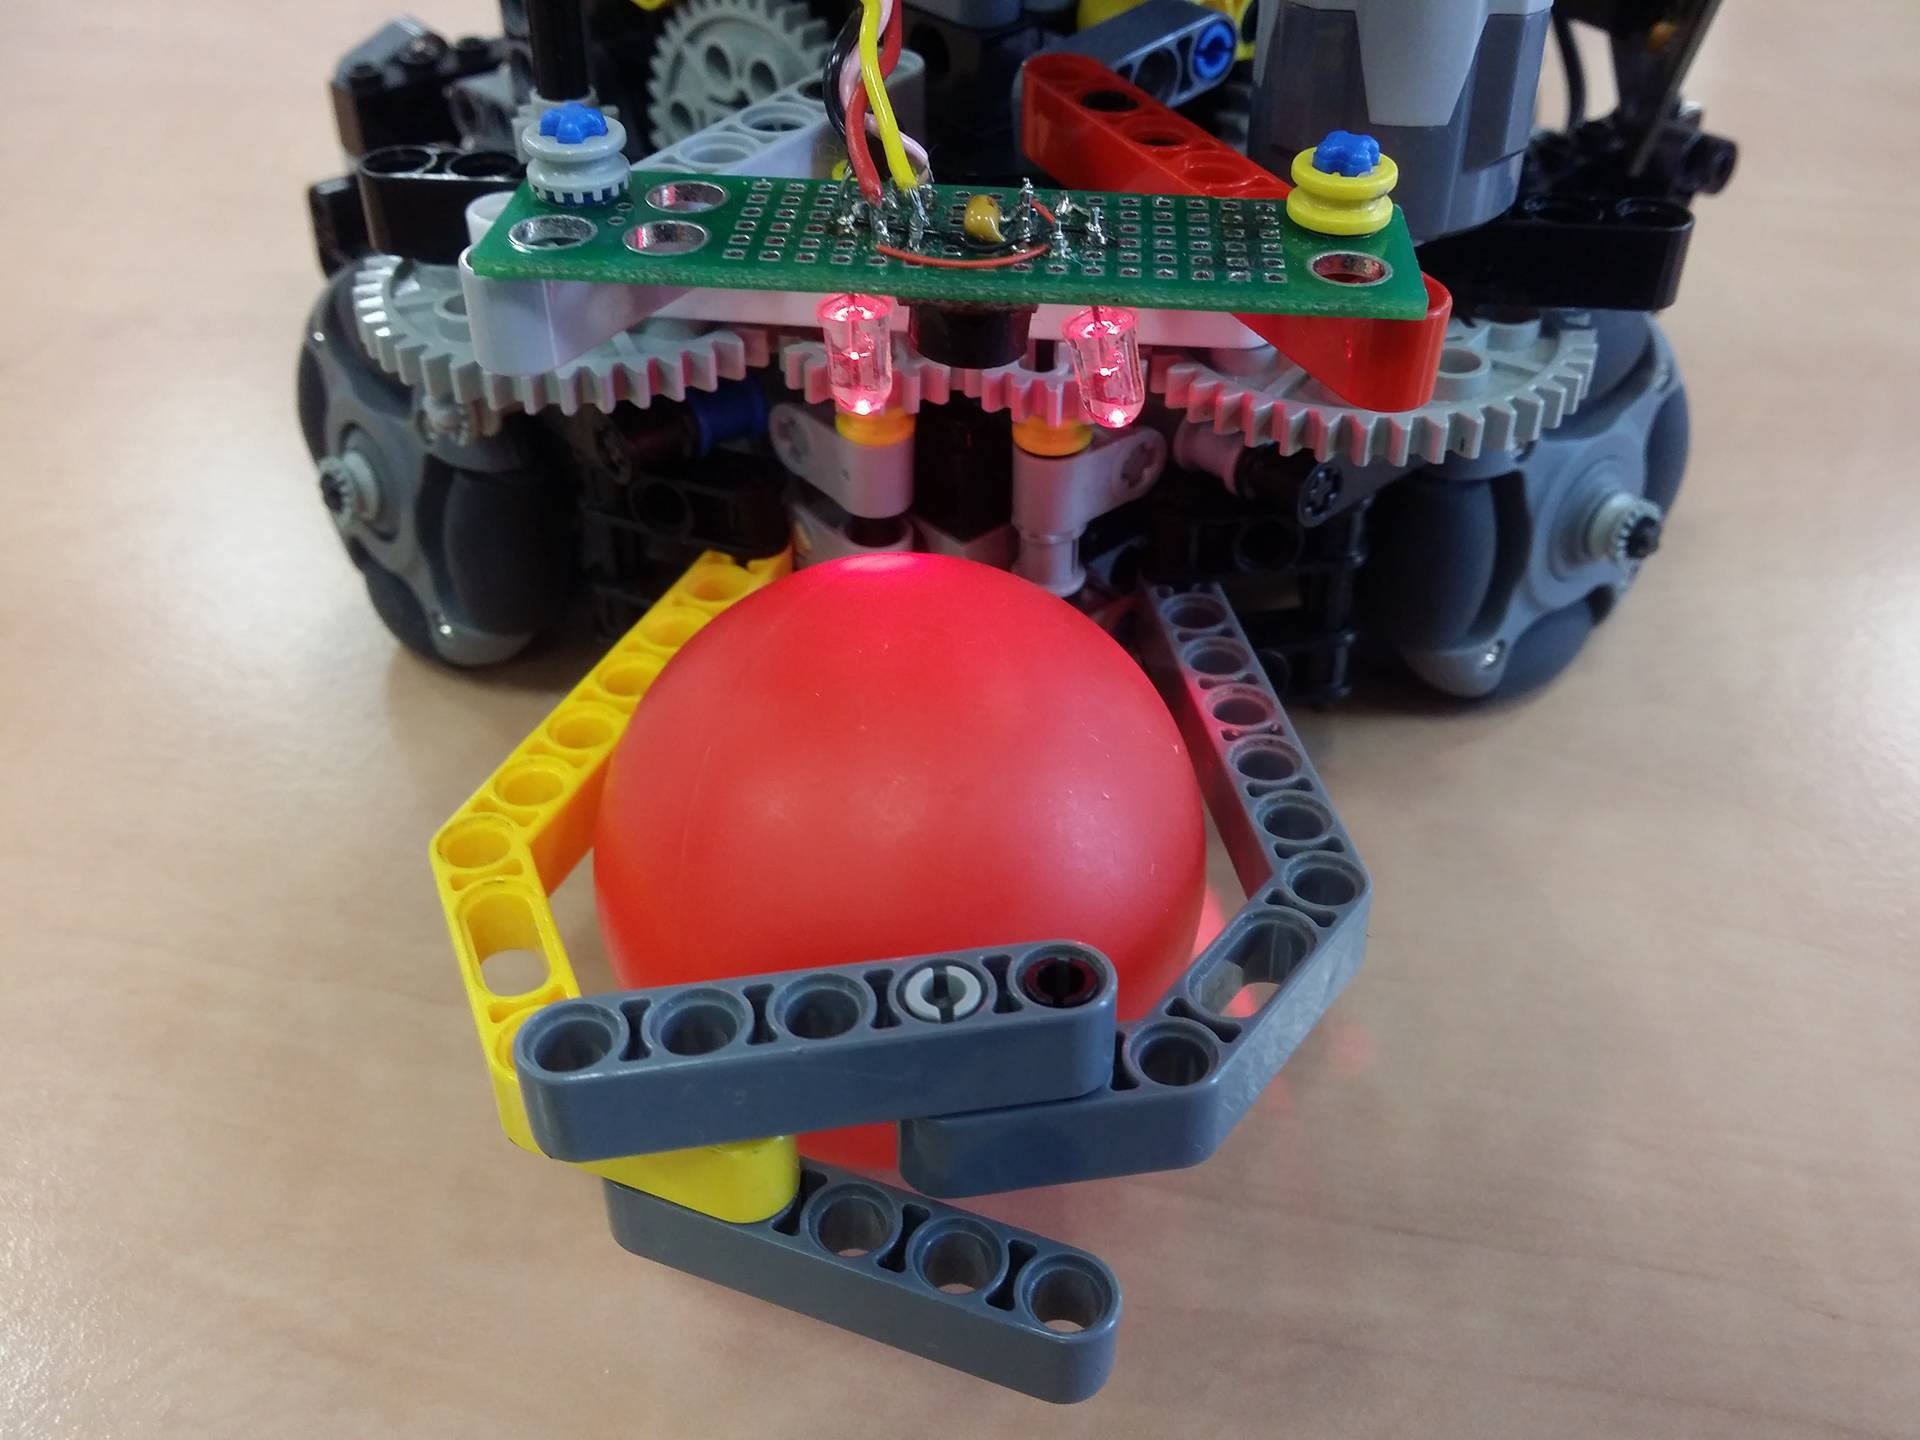
\includegraphics[scale=.1]{sensor1}
\caption{The light sensor with the ball grabbed}
\label{fig:sensor}
\end{figure}

\end{document}
